% %%%%%%%%%%%%%%%%%%%%%%%%%%%
% % Systematic uncertainties
% %%%%%%%%%%%%%%%%%%%%%%%%%%%

 
% \section{Systematic uncertainties \label{sec:systematics}}
% The input to the statistical analysis is an ensemble of histograms in the $(\mathrm{M_R},
% \mathrm{R^2})$ plane that  incorporate systematic uncertainties in the simulated signal and
% background samples.   The independent systematic effects, described below, are sampled
% simultaneously. For each sampled systematic effect, the same
% zero mean, unit variance, Gaussian variate is used in the calculation 
% of the random shift of the systematic effect
%  for all the signal and background models.
% Likewise the same randomly sampled parton distribution functions (PDF) are used for all signal and
% background models. In this way, the statistical dependencies among all bins of the signal and
% background models are correctly, and automatically, modelled. The sampling of the systematic effects
% is repeated several hundred times.  
%  
% In all cases, except for the PDFs, the systematic uncertainties are in the scale factors (SF) 
% applied to the simulated samples to correct them for modelling deficiencies. We consider the
% systematic uncertainties of the following quantities:
% 
% \begin{itemize}
% 
% \item {\bf Jet energy scale:}   The uncertainties are dependent on jet \pt and $\eta$.  
% 
% \item {\bf Parton distribution functions:} We use 100 randomly sampled sets of PDFs from {\tt
% NNPDF23\_lo\_as\_0130\_qed}~\cite{nnpdf},  {\tt MSTW2008lo68cl}~\cite{Martin:2009iq}, and {\tt
% CT10}~\cite{Lai:2010vv}.  The samples for the latter two are generated using the program
% {\tt hessian2replicas}, recently
% released with {\tt LHAPDF6}~\cite{LHAPDF6}. Given a sampled set $i$, for PDF set $K$ and the
% PDF set $O$ with which the events were simulated, events are reweighted using the scale factors,
% ${\rm SF}_{K, i} = w_{K, i} / w_{O}$,
% where the weights $w$ are products of the event-by-event PDFs for the colliding partons.
% 
% \item {\bf Trigger efficiency: }  We take the uncertainty in each bin, as a function of $H_T$ and
% leading jet $\pt$, to be the maximum of the statistical uncertainty in the efficiency after
% preselection and the difference between the efficiencies before and after preselection. 
% 
% \item {\bf $\cPqb$ tagging scale factors:} The $\cPqb$ tagging performance differs between data and
% simulation, and differs between the CMS full simulation (FullSim) and the parametric simulation
% (FastSim).  The simulated events are therefore corrected by applying  jet flavour, \pt, and $\eta$
% dependent data / FullSim and FullSim / FastSim $\cPqb$ tag scale factors.
% 
% \item {\bf $\PW$ tagging scale factors:} The $\PW$ boson tag efficiency, and the misidentification
% (or \textit{fake}) rate for $\PW$ boson tag, $\PW$ boson mass-tag, and $\PW$ boson anti-tag differ
% between data and simulation, as well as between FullSim and FastSim.  Data / FullSim and FullSim /
% FastSim scale factors,  whose uncertainties are functions of jet $\pt$, are applied to the simulated
% samples.  Some of these scale factors are derived specifically for this study  and are described
% further in Section~\ref{sec:Wtag_SF}.
% 
% \item {\bf Lepton ID:} For electrons, we use \pt and $\eta$-dependent scale factors. The 
% uncertainties
% are also \pt and $\eta$-dependent.  The corresponding uncertainties for muons are negligible.  
% 
% \item {\bf Initial State Radiation:} Deficiencies in the modelling of initial-state-radiation (ISR) 
% are corrected by reweighting~\cite{ISRerr} the signal samples using an event weight 
% that depends on the \pt of the recoiling system.  The associated systematic uncertainty is equal to
% the difference $1 - w_{ISR}$, where $w_{ISR}$ is the ISR event weight.  
% 
% \item {\bf Top quark transverse momentum:} Differential top-quark-pair cross section analyses have
% shown that the shape of the \pt spectrum of  top quarks in data is softer than
% predicted~\cite{toppt}. To account for this, we reweight events  based on the \pt of the generator
% level $t$ and $\bar{t}$ quarks in the $t\bar{t}$ simulation.  
% The uncertainty associated with this reweighting is taken to be equal to the full size of the
% reweighting.
% 
% \item {\bf Pileup: } Simulated events are reweighted so that their pileup (\ie  vertex multiplicity)
% distributions  and the observed pileup distribution,  match. The minbias cross section is varied by
% $\pm 5\%$, thereby changing the shape of pileup distribution and therefore the weights.  The
% difference in weights is taken as a measure of the uncertainty in the pileup distribution.  
% 
% \item {\bf QCD spectrum:} The cross checks described in Section~\ref{sec:selection} showed that
% there is a 40\% uncertainty in the QCD multijet scale factor $\kappa$ between the signal and QCD
% regions.  This uncertainty is accounted for by including an additional 33\% uncertainty to the
% $\kappa$
% parameters, as described in Section~\ref{sec:likelihood}.
% 
% \item {\bf $\cPZ (\rightarrow \nu \nu)+$jets prediction:} About 8\% of the background in the signal
% region is composed of $Z(\rightarrow\nu\nu)$+jets events. Since we require the presence of at least
% one $\cPqb$ tagged jet, and given the known deficiency in modelling $\cPZ$ production in association
% with heavy flavour, we include an extra systematic uncertainty in the $\cPZ(\rightarrow\nu\nu)$+jets
% contribution.  This uncertainty is estimated using a data control region enriched in
% $\cPZ(\rightarrow \ell \bar{\ell})+$jets, required to have exactly two tight leptons, same flavour
% and opposite sign ($e$ or $\mu$), $60 < m_{ll} < 120\GeV$, at least one $\cPqb$ tagged jet, and at
% least one $\PW$ mass-tagged jet.  We estimate the uncertainty by first computing bin-by-bin data/MC
% ratios in this control region.  Then, we take the uncertainty in the ratio in each bin as the
% standard deviation of a Gaussian, normalized to  the number of events in that bin.  Finally, the
% Gaussians from all bins are superposed, and the 
% uncertainty is taken to be the magnitude of the 68\% band around a ratio of unity.
% 
% \end{itemize}
% 
% As noted above, all systematic effects are varied simultaneously. However, in order to see the
% effect of each systematic uncertainty individually, each systematic effect $i$ is varied by $\pm
% \delta_i$.  The effect on the background and signal samples in the signal region is shown in
% Table~\ref{tab:bgsigsys}.  The signal values are obtained from averaging over all mass points in the
% {\it T1ttcc} ($\Delta m = 25\GeV$) plane.  The PDF systematic uncertainties are obtained by running
% over 100 different PDF set members, fitting a Gaussian to the efficiency distribution and taking the
% width of the Gaussian.  The last line in the table corresponds to the full sampling of the
% systematic uncertainties. To obtain this value we again fit a Gaussian to the efficiency
% distribution obtained from the full systematic sampling including 500 variations.  We note  that,
% although the effects of some of these systematic uncertainties on the backgrounds are large, these
% do not influence our results greatly because only the 
% ratios of simulated background counts enter the statistical analysis, not the distributions
% themselves.  Therefore, most of the systematic effects cancel.  The dominant systematic uncertainty
% arises from the parton distribution functions. The statistical precision of the control regions is
% the leading uncertainty for the search bins at large $\mathrm{M_R}$ or $\mathrm{R^2}$.
% 
% {
%\renewcommand{\arraystretch}{1.4}
\begin{table}[htpb]
\centering
\caption{Summary of $\pm 1 \sigma$ systematic uncertainties for the average signal count of all {\it T1ttcc} ($\Delta m=25\GeV$) signal points, and for the total background count in the signal region, unless indicated otherwise, as determined from simulation.  \label{tab:bgsigsys}}
\vspace{1ex}
\begin{tabular}{l c c}
\toprule
Systematic Effect & Signal up down & Background up down \\
\midrule
JEC & $ +2.2\% -2.1\%$   & $ +10.9\% -5.2\%$\\ 
Trigger & $ +1.1\% -3.3\%$ & $ +3.4\% -5.7\%$\\
b tag FullSim & $ +2.1\% -2.3\%$& $+3.9\% -4.0\%$\\
b tag FastSim & $ +1.2\% -1.3\%$& - \\
W tag efficiency Fullsim & $ +9.0\% -8.9\%$& $+4.6\% -4.6\%$\\
W tag efficiency FastSim & $ +2.2\% -2.2\%$& - \\
W tag fake rate FullSim & - & $ +1.4\% -1.4\%$ \\
W anti-tag fake rate FullSim ($Q$ region only) & - & $+2.6\% -2.6\%$ \\ 
W mass-tag fake rate FullSim ($W$ region only) & - & $+2.3\% -2.3\%$ \\ 
Electron ID ($T$ and $W$ region only) & - & $+0.2\% -0.2\%$ \\ 
Pileup & $ +0.5\% -0.5\%$ & $+1.0\% -1.1\%$\\
ISR & $ +6.6\% -6.6\%$ & - \\
Top \pt spectrum & - & $ -14.4\% ~ 20.5\%$ \\
$\cPZ\rightarrow\nu\nu+$ heavy flavour  & - & $+4.0\% -4.0\%$ \\
PDF & $20.7\%$ &  $10.7\%$ \\
\midrule
All &  $24.4\%$ &  $22.1\%$ \\
\bottomrule
\end{tabular}
\end{table}
}
 




% 
% 
% %%%%%%%%%%%%%%%%%%%%%%%%%%%%%%%%%%%%%%%%%%%%%%%%%%%%%%%%%%%%%%%%%%%%%%%%%%%%%%%%%%%%%%%%%%%%%%%%
% 
% In this section the considered systematic uncertainties will be discussed. 
% 
% \subsection{Jet energy corrections (JEC) \label{sec:JEC}}
% 
% Jet energy corrections are a set of tools that allow the proper mapping of the measured jet energy
% deposition to the analysis-desired level (particle or parton).  
% CMS factorizes the effects of different corrections, and defines JEC in levels applied sequentially.
%  
% Each level of correction is a scaling of the 4-jet momentum by a scale factor (correction) which
% depends on various jet related quantities such as \pt, $\eta$ and flavor.  
% 
% Uncertainties on JEC come from various uncorrelated sources.   
% Given there are $M$ such sources, the correction on a jet's \pt becomes 
% \begin{equation}
% s(\pt, \eta, \alpha_i) = \sum_{i=1}^M \alpha_i S_i (\pt, \eta)
% \end{equation}
% where $S_i (\pt, \eta)$ is a \pt and $\eta$-dependent JEC uncertainty for a source $i$ and
% $\alpha_i$s are weights randomly sampled from Gaussian distributions with mean 0 and width 1.  
% Here, $\alpha_i$ are different for each source, but are universal for each jet and each event.  
% In a much simpler approach JEC corrections can be computed as
% \begin{equation}
% s(\pt, \eta, \alpha) = \alpha S (\pt, \eta) = \alpha \sqrt {\sum_i^M s_i^2 (\pt, \eta) }
% \end{equation}
% using a total uncertainty $S (\pt, \eta)$ and a random number from a single Gaussian.  
% The jet $p_T$s are corrected as:
% \begin{equation}
% \pt^{data} = (1 + s(\pt, \eta, \alpha)) \pt^{MC}.
% \end{equation}
% This calculation is repeated $N$ times, each time, using a different number sampled from the
% Gaussian.  
% The overall effect of JEC uncertainty on the yield is obtained from the distribution of resulting
% $N$ yields.  
% The JEC uncertainties are also propagated to \ETm .
% % (technical method: use TLorentzVectors: \ETm - sumuncorrected + sumcorrected).
% 
% %%%%%%%%%%%%%%%%%%%%%%%%%%%%%%%%%%%%%%%%%%%%%%%%%%%%%%%%%%%%%%%%%%%%%%%%%%%%%%%%%%%%%%
% 
% \subsection{Parton distribution functions (PDF) \label{sec:PDFweights}}
% 
% In order to evaluate the systematics on parton distribution functions (PDFs), we use the three
% recommended PDF sets {\tt CT10}, {\tt MSTW2008lo68cl} and {\tt NNPDF23\_lo\_as\_0130\_qed} by
% PDF4LHC.  
% Since we take into account full correlations wihtin systematic variations, we need a way to sample
% randomly from the PDF uncertainties.  Of the three recommended PDF sets, NNPDF presents the PDF
% eigenvectors as a randomly distributed set, while the other groups provide eigenvectors obtained by
% varying the PDF fit parameters by $\pm 1$ standard deviation.  
% However, the recently developed {\tt LHAPDF6} offers a formal way to convert the latter sets into
% randomly distributed sets.  
% We have used the {\tt examples/hessian2replicas} code provided in {\tt LHAPDF6} to generate randomly
% distributed PDF sets with 100 members each for {\tt CT10} and {\tt MSTW2008lo68cl}.  
% 
% Given a member $i$ of a PDF set $K$, we calculate a scale factor for each event as the ratio of the
% PDF weight computed using the member $i$ and the weight computed using the central value of the
% original PDF used for generating the event
% \begin{equation}
% {\rm SF}^{\rm PDF}_{K}(i) = w^{\rm PDF}_{K}(i) / w^{\rm PDF}_{\rm orig}(\rm central)
% \end{equation} 
% All SM samples except for those generated with {\tt POWHEG} and all SMS signal samples were
% generated using {\tt CTEQ6.1}, while all {\tt POWHEG} samples were generated using {\tt CT10}.
% 
% The overal PDF uncertainty is then obtained from the distribution of ${\rm SF}^{\rm PDF}_{K}(i)$s
% obtained by a random selection of $K$s and $i$s.  
% 
% To study the effect of the different PDF sets on the MC counts used in the background estimation, we
% compute the MC counts using a random selection of PDF members from the three PDF sets. A Gaussian
% function is then fitted to these distributions. 
% Figures~\ref{fig:PDF_effect_on_bg_QCD}-\ref{fig:PDF_effect_on_bg_oth2} show the result of this
% procedure for the various considered MC counts. 
% There is a Gaussian distribution for each PDF set, and the arrow indicates the value obtained using
% the PDF that was used during the generation of the MC samples. From this we can see that the overall
% systematic uncertainty from parton distribution functions on the background counts is due to both
% the difference in the nominal values of the PDF sets, and the spread within the separate PDF sets. 
% Figure~\ref{fig:PDF_effect_on_sig} shows the equivalent for an example signal point. Here we see
% that the {\tt CT10} spread dominates the total uncertainty. 
% 
% \begin{figure}[p]
% \centering
% 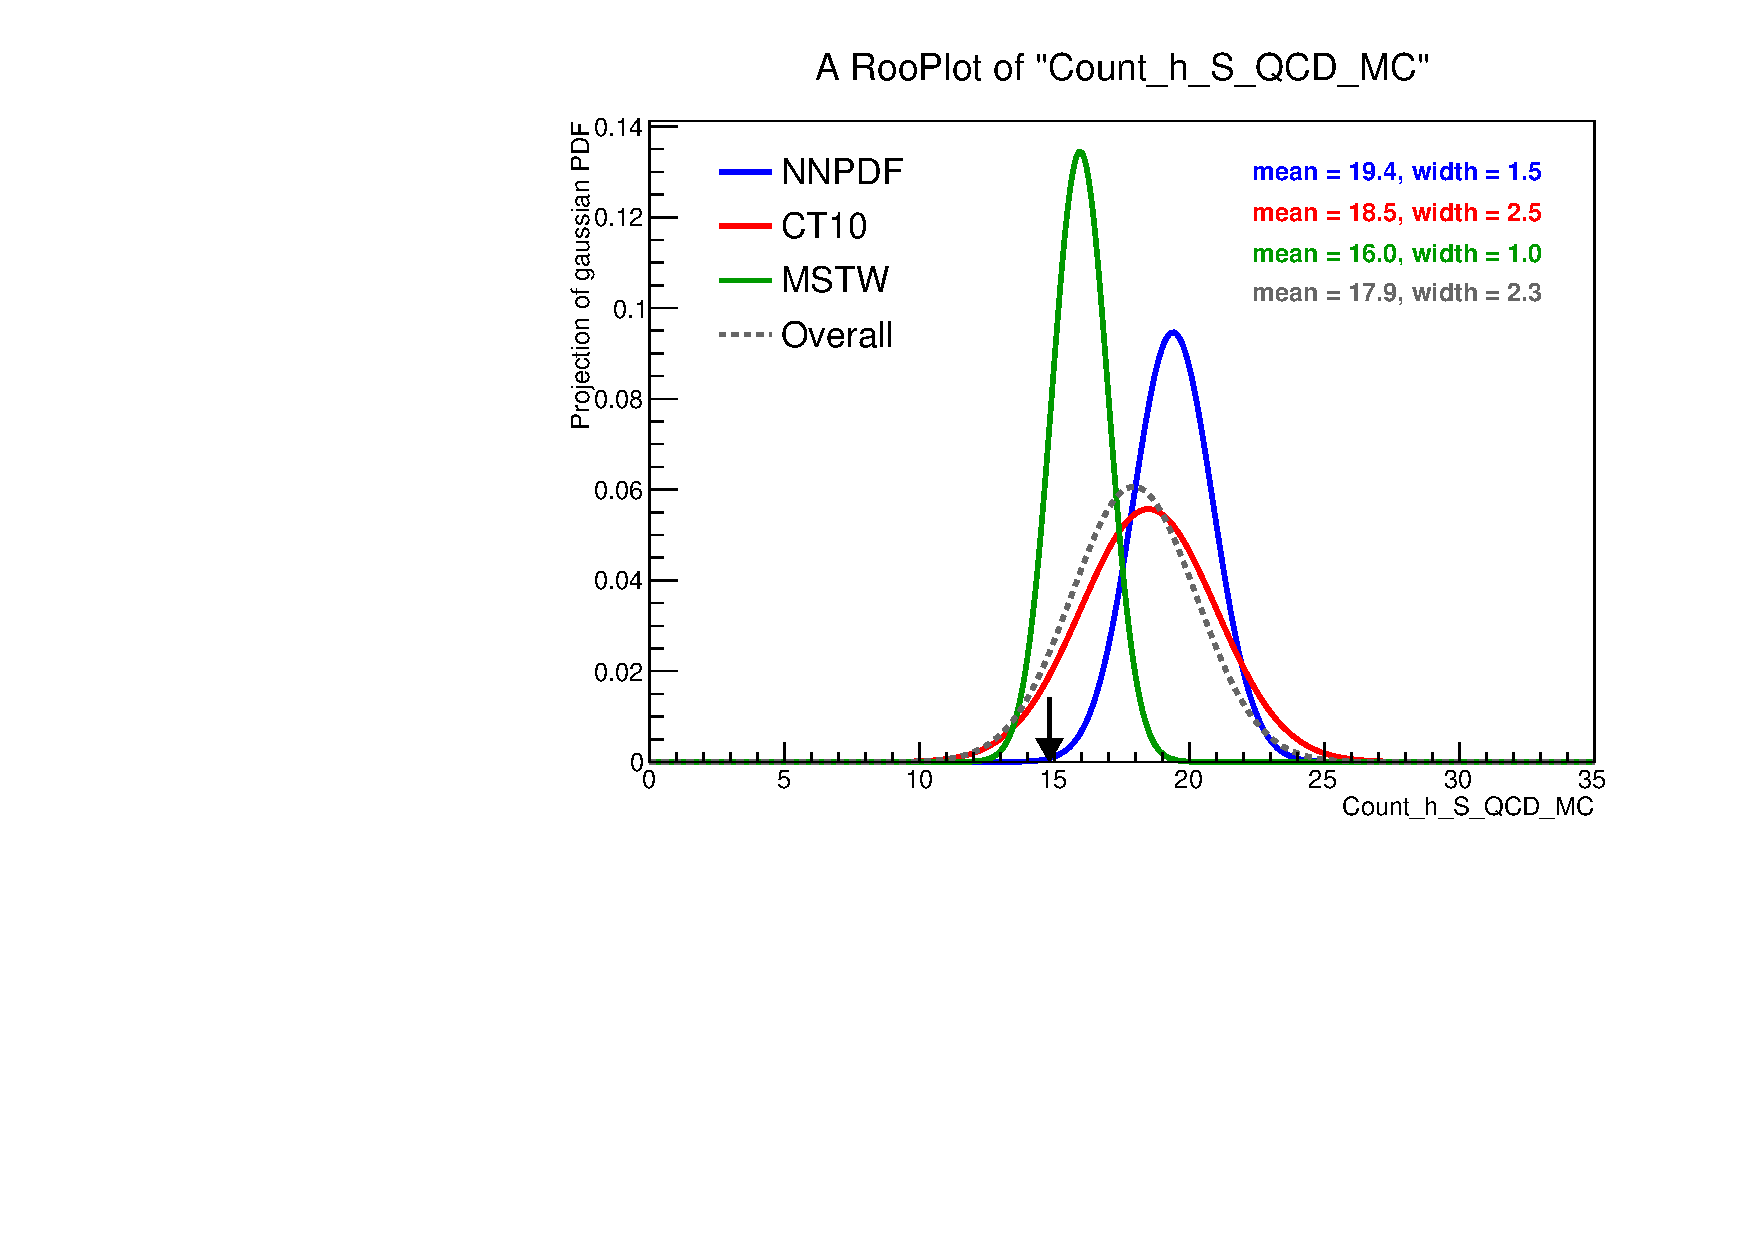
\includegraphics[width=0.49\textwidth]{figures/Systematics/PDF/h_S_QCD_MC}
% 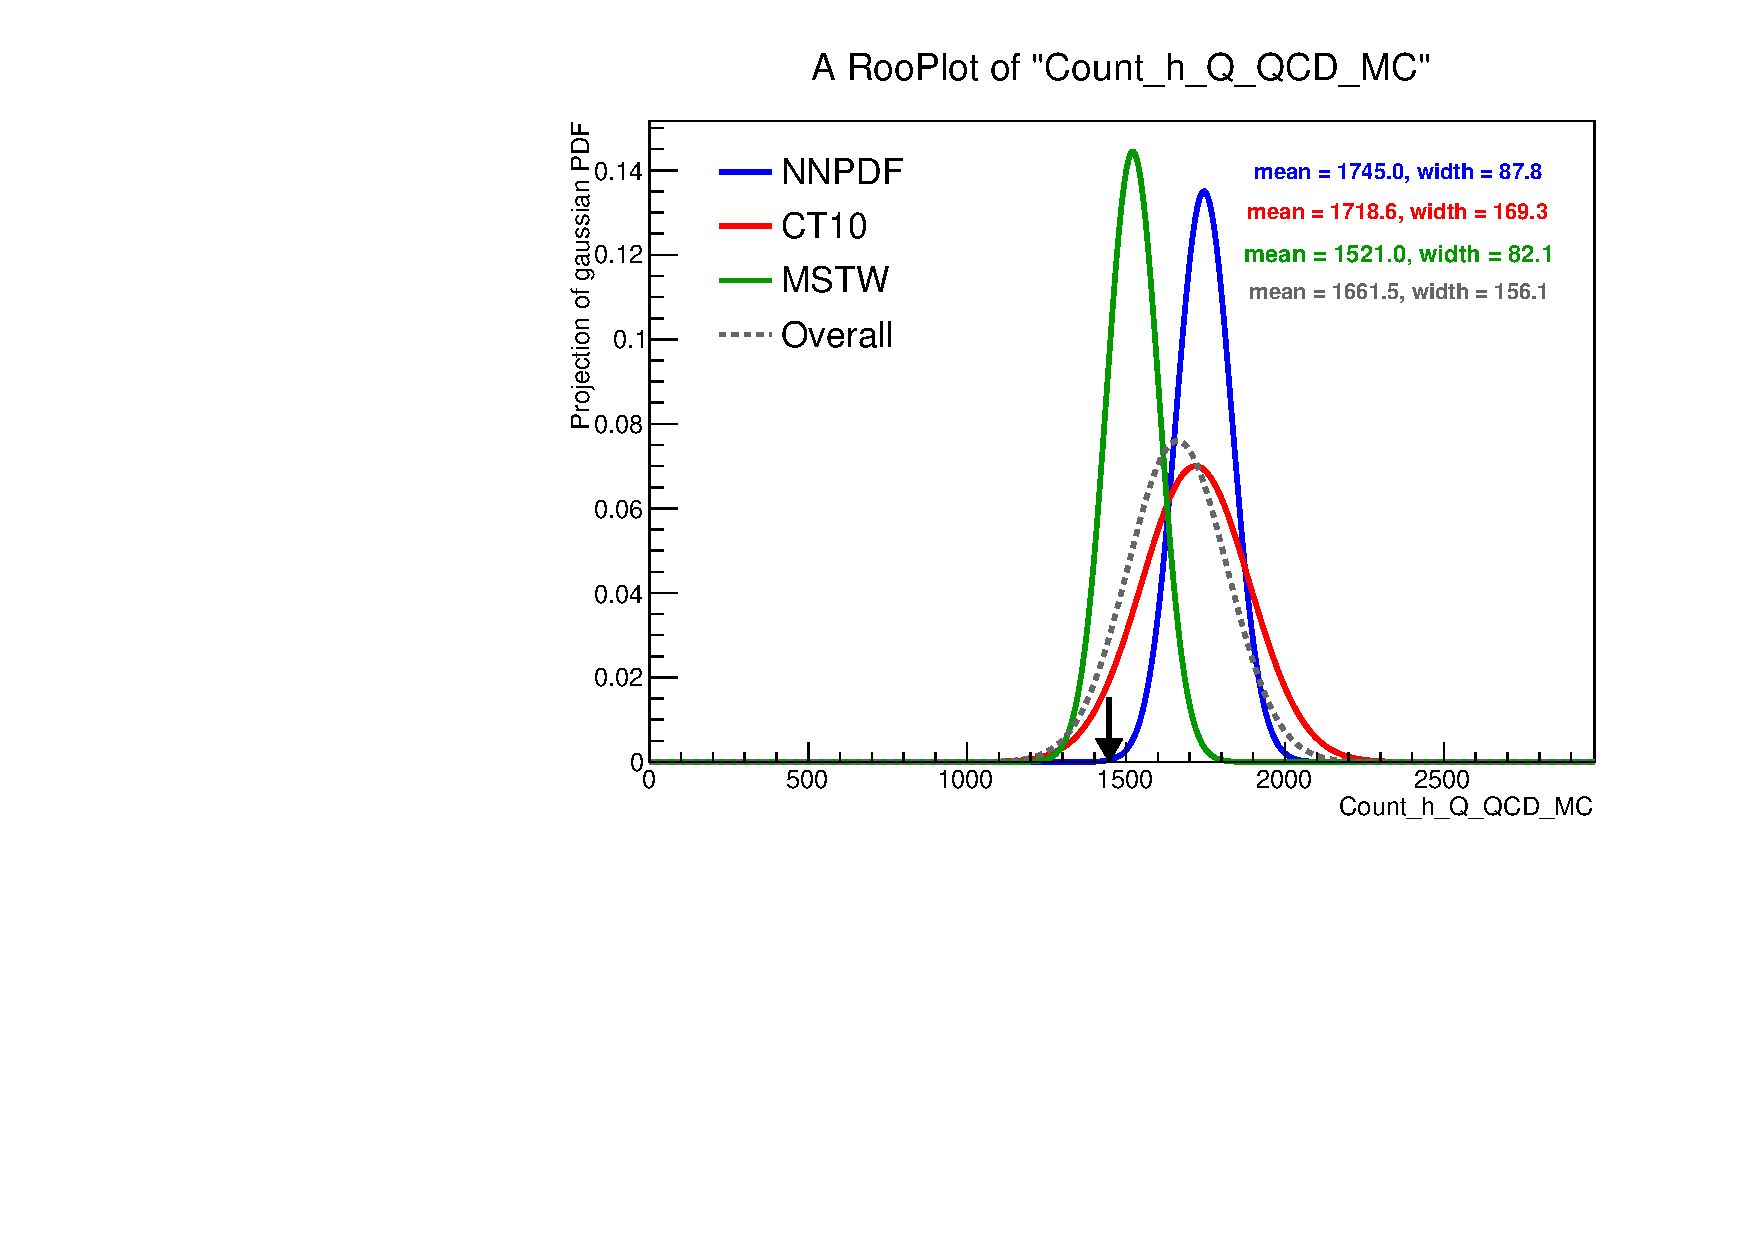
\includegraphics[width=0.49\textwidth]{figures/Systematics/PDF/h_Q_QCD_MC}
% \caption{Influence of different PDF sets on the MC counts entering $\kappa_{QCD}^{Q/S}$
% \label{fig:PDF_effect_on_bg_QCD}}
% \end{figure}
% 
% \begin{figure}[p]
% \centering
% 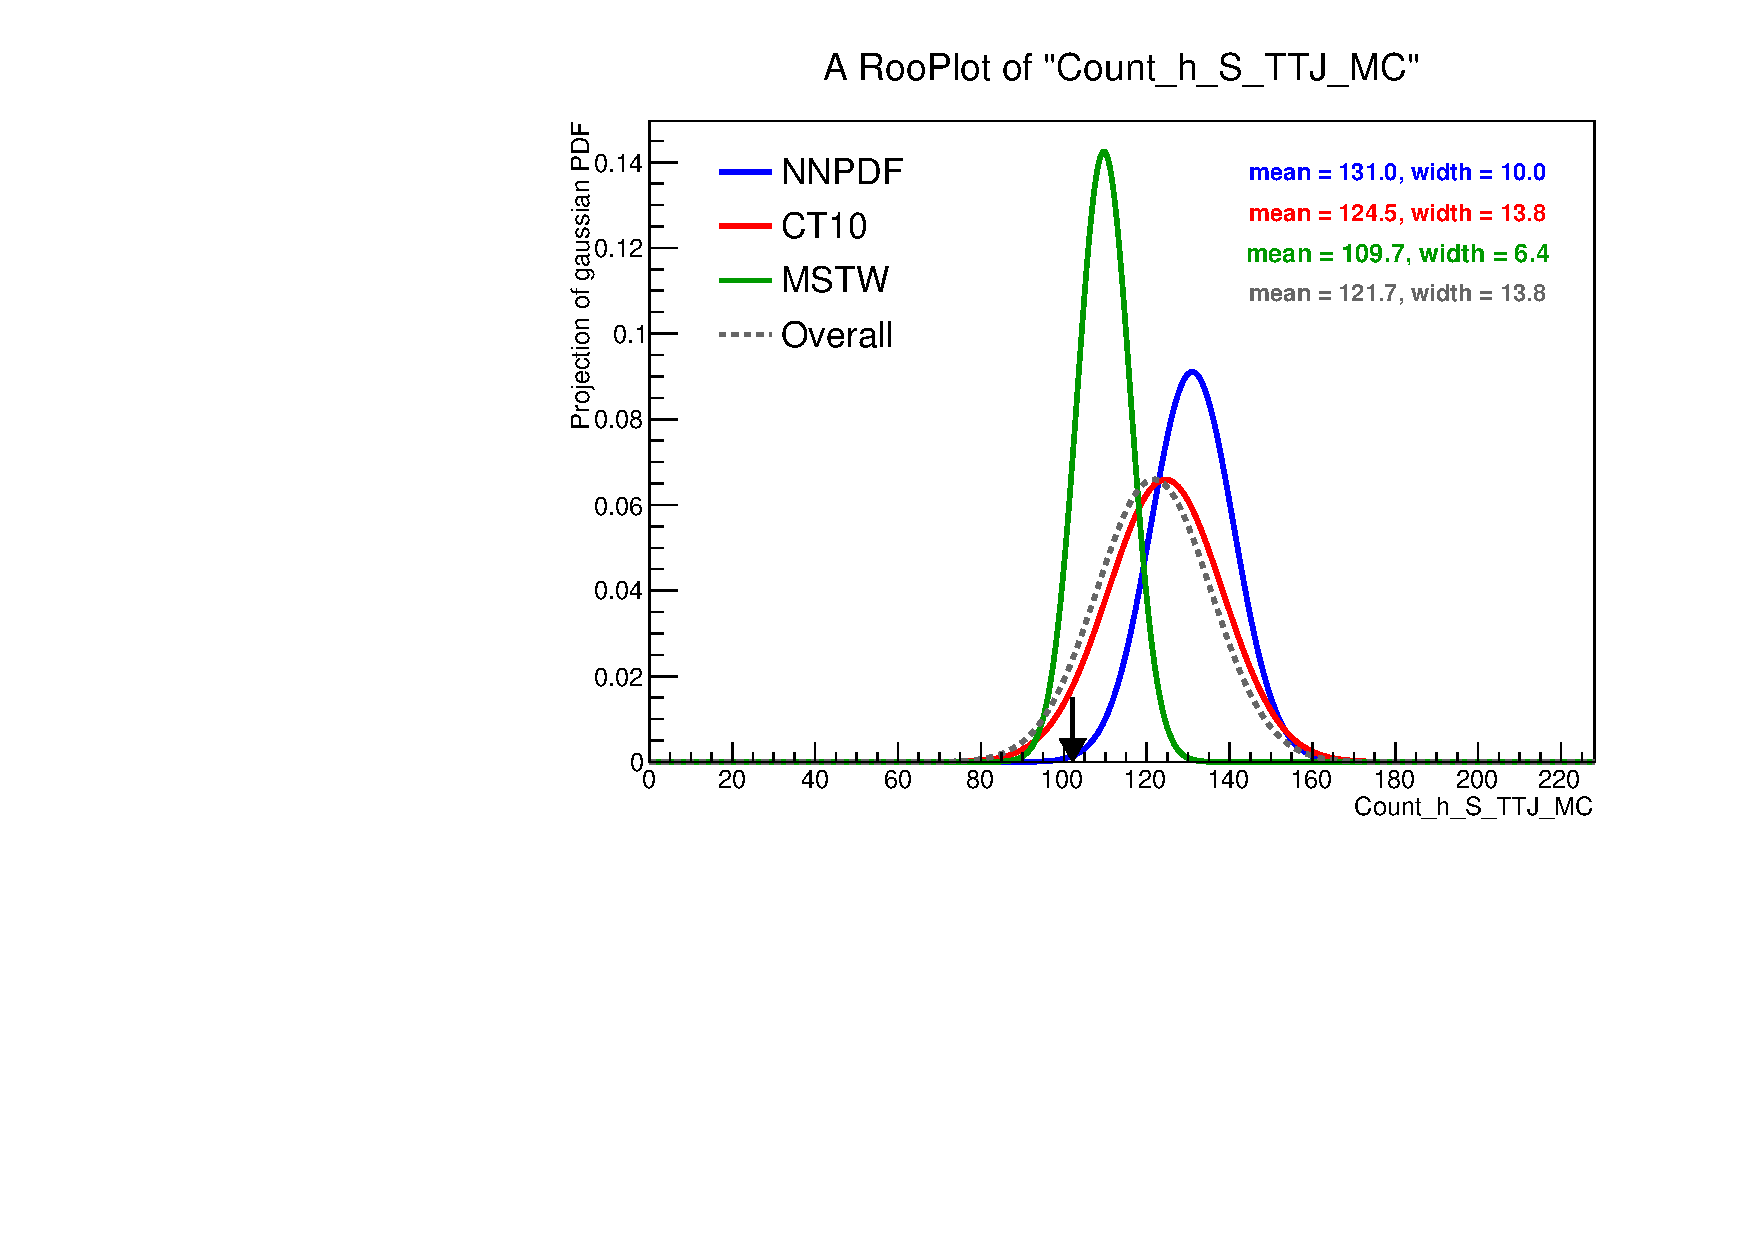
\includegraphics[width=0.49\textwidth]{figures/Systematics/PDF/h_S_TTJ_MC}
% 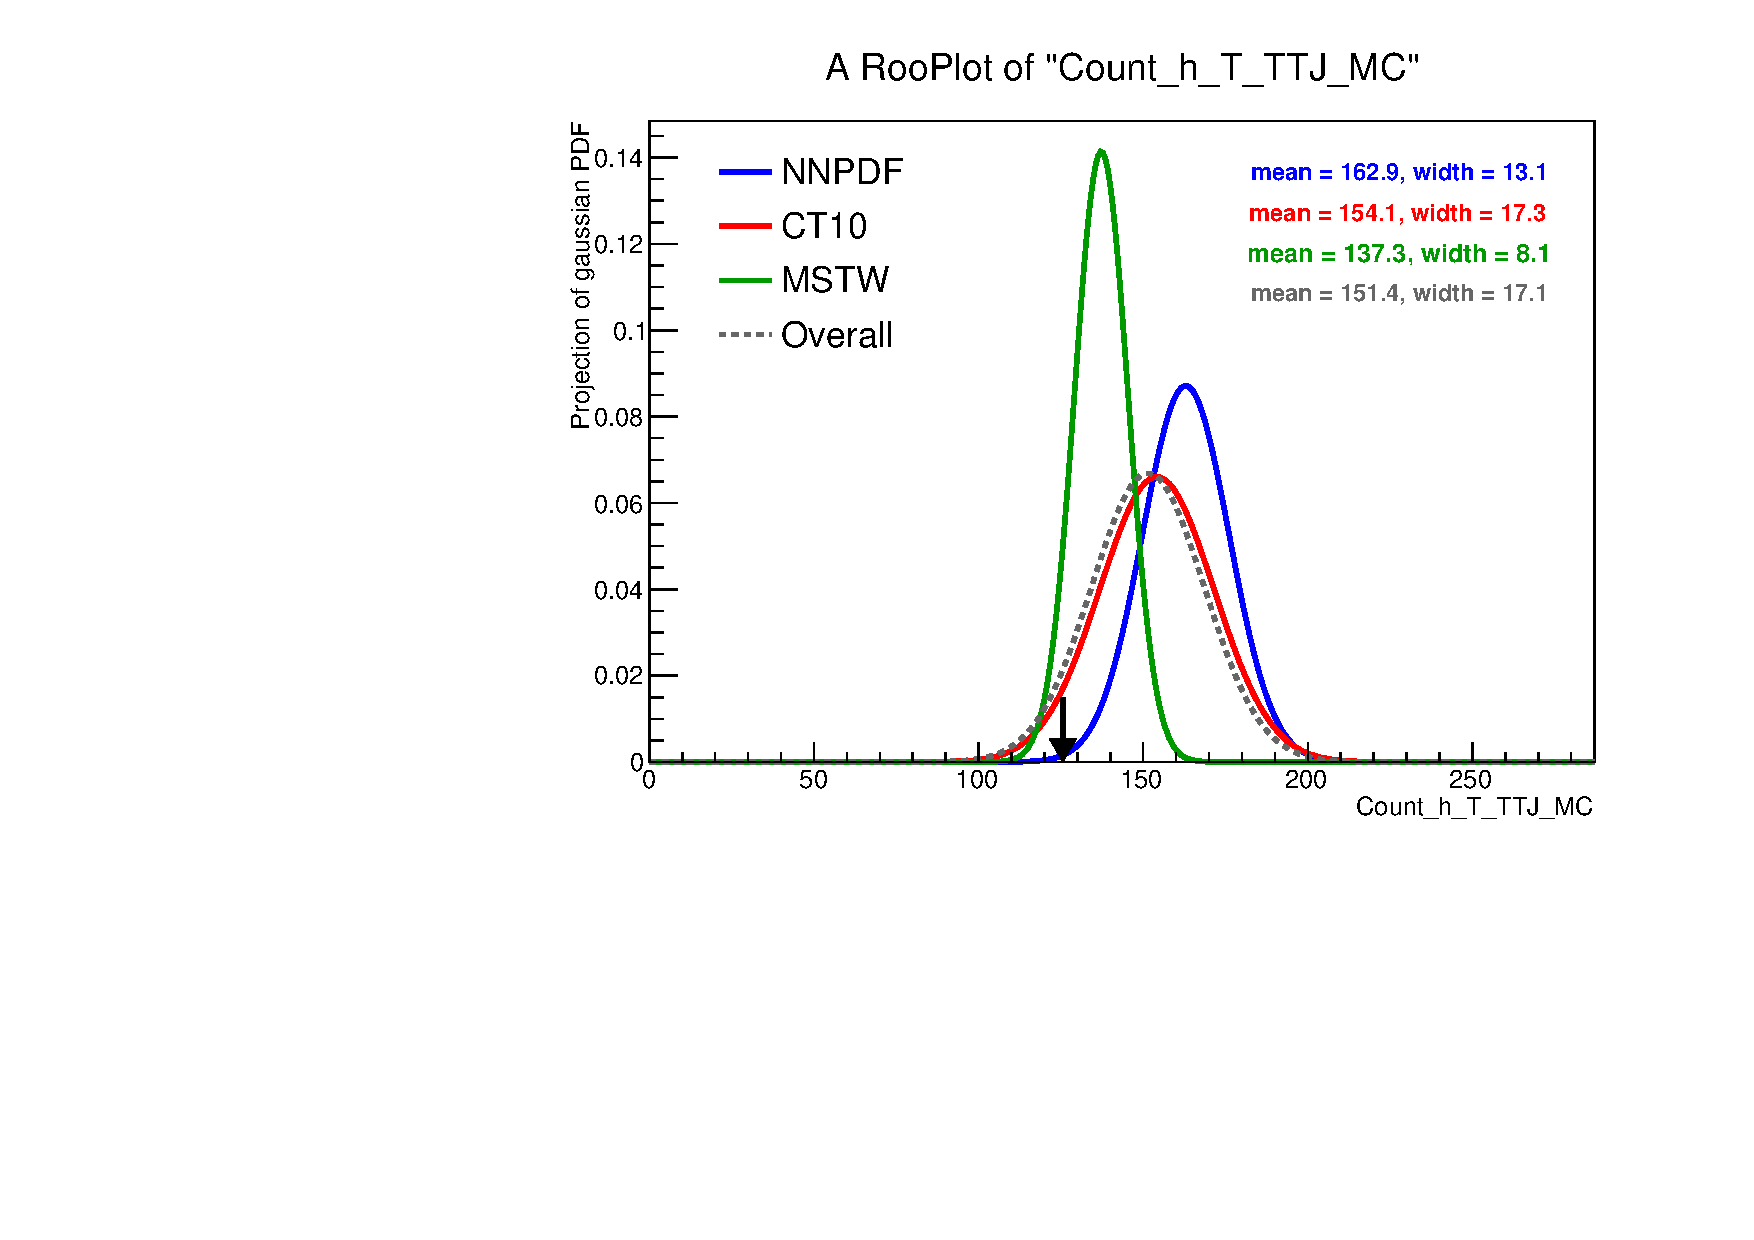
\includegraphics[width=0.49\textwidth]{figures/Systematics/PDF/h_T_TTJ_MC}
% \caption{Influence of different PDF sets on the MC counts entering $\kappa_{TTJ}^{T/S}$
% \label{fig:PDF_effect_on_bg_TTJ}}
% \end{figure}
% 
% \begin{figure}[p]
% \centering
% 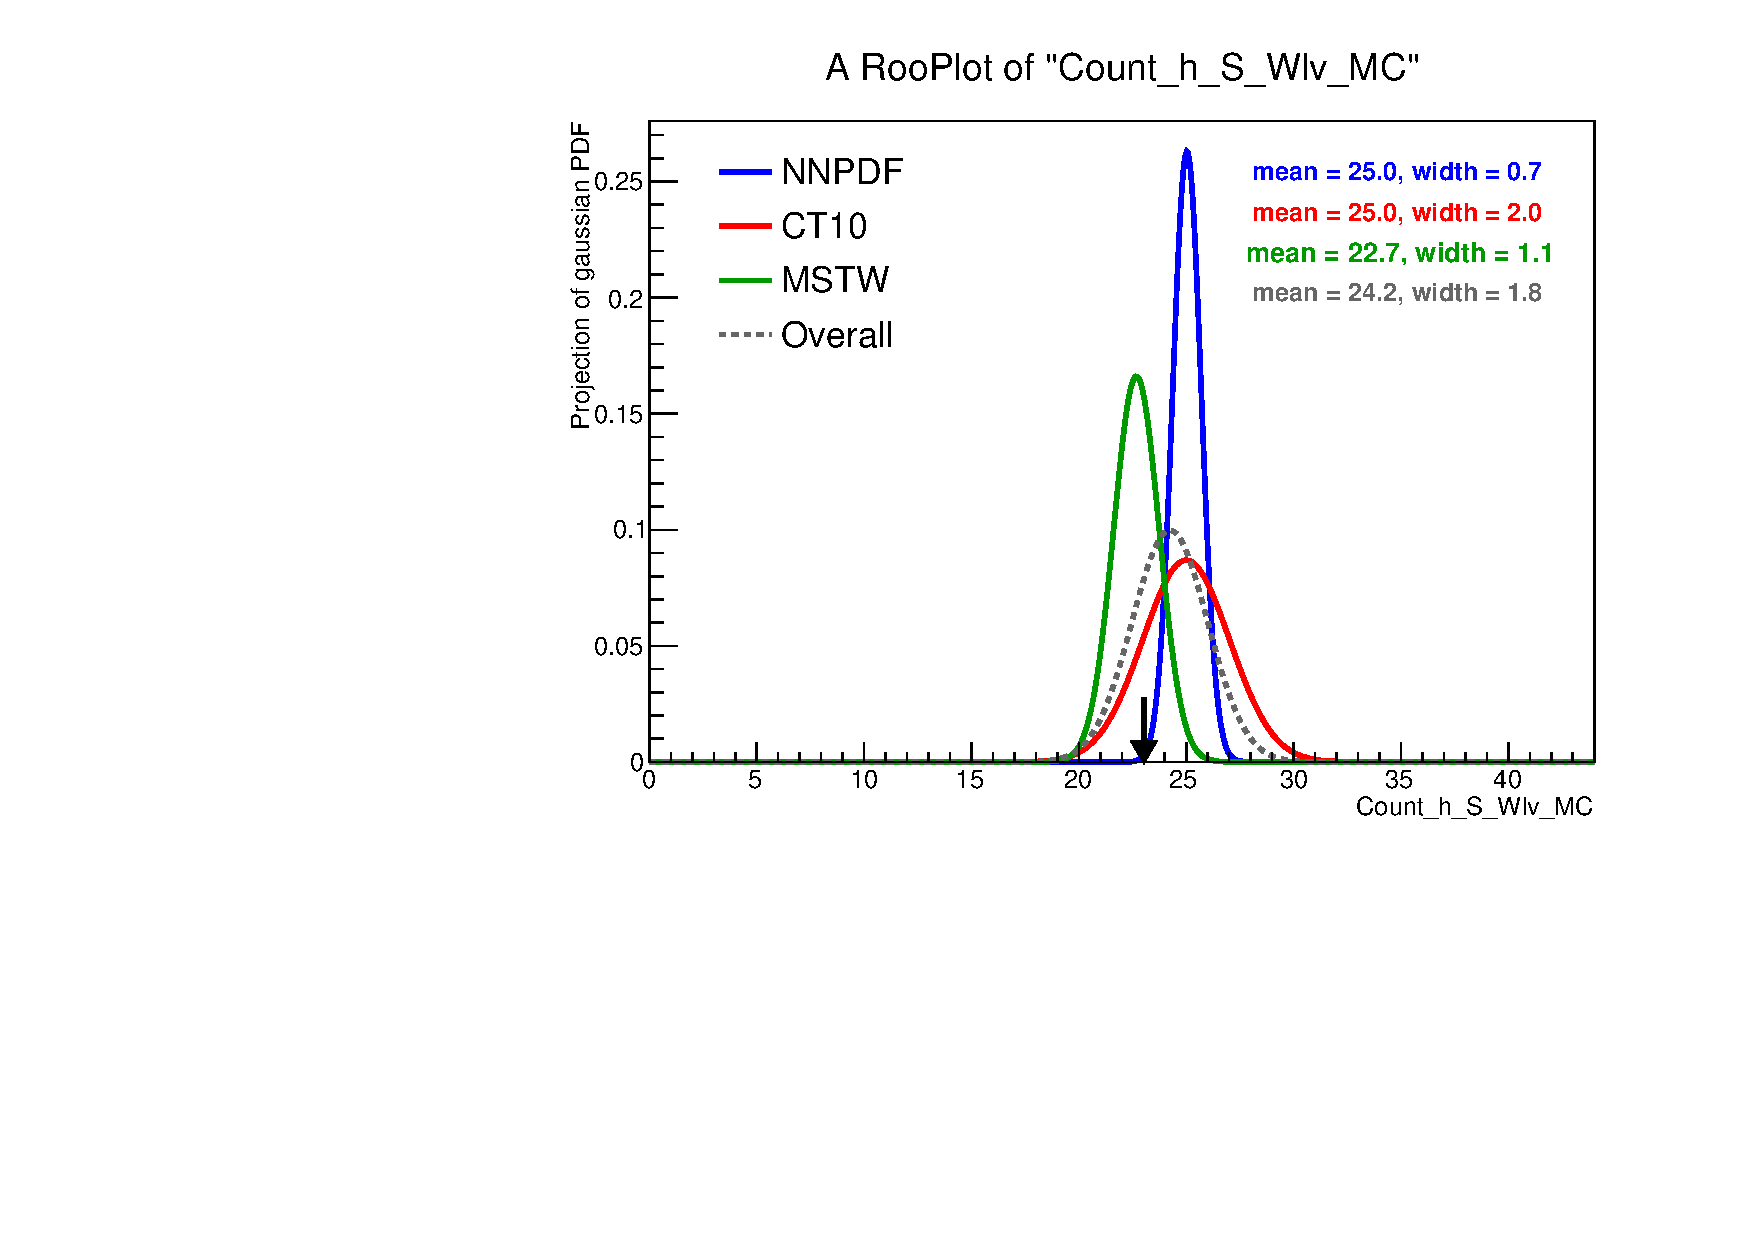
\includegraphics[width=0.49\textwidth]{figures/Systematics/PDF/h_S_Wlv_MC}
% 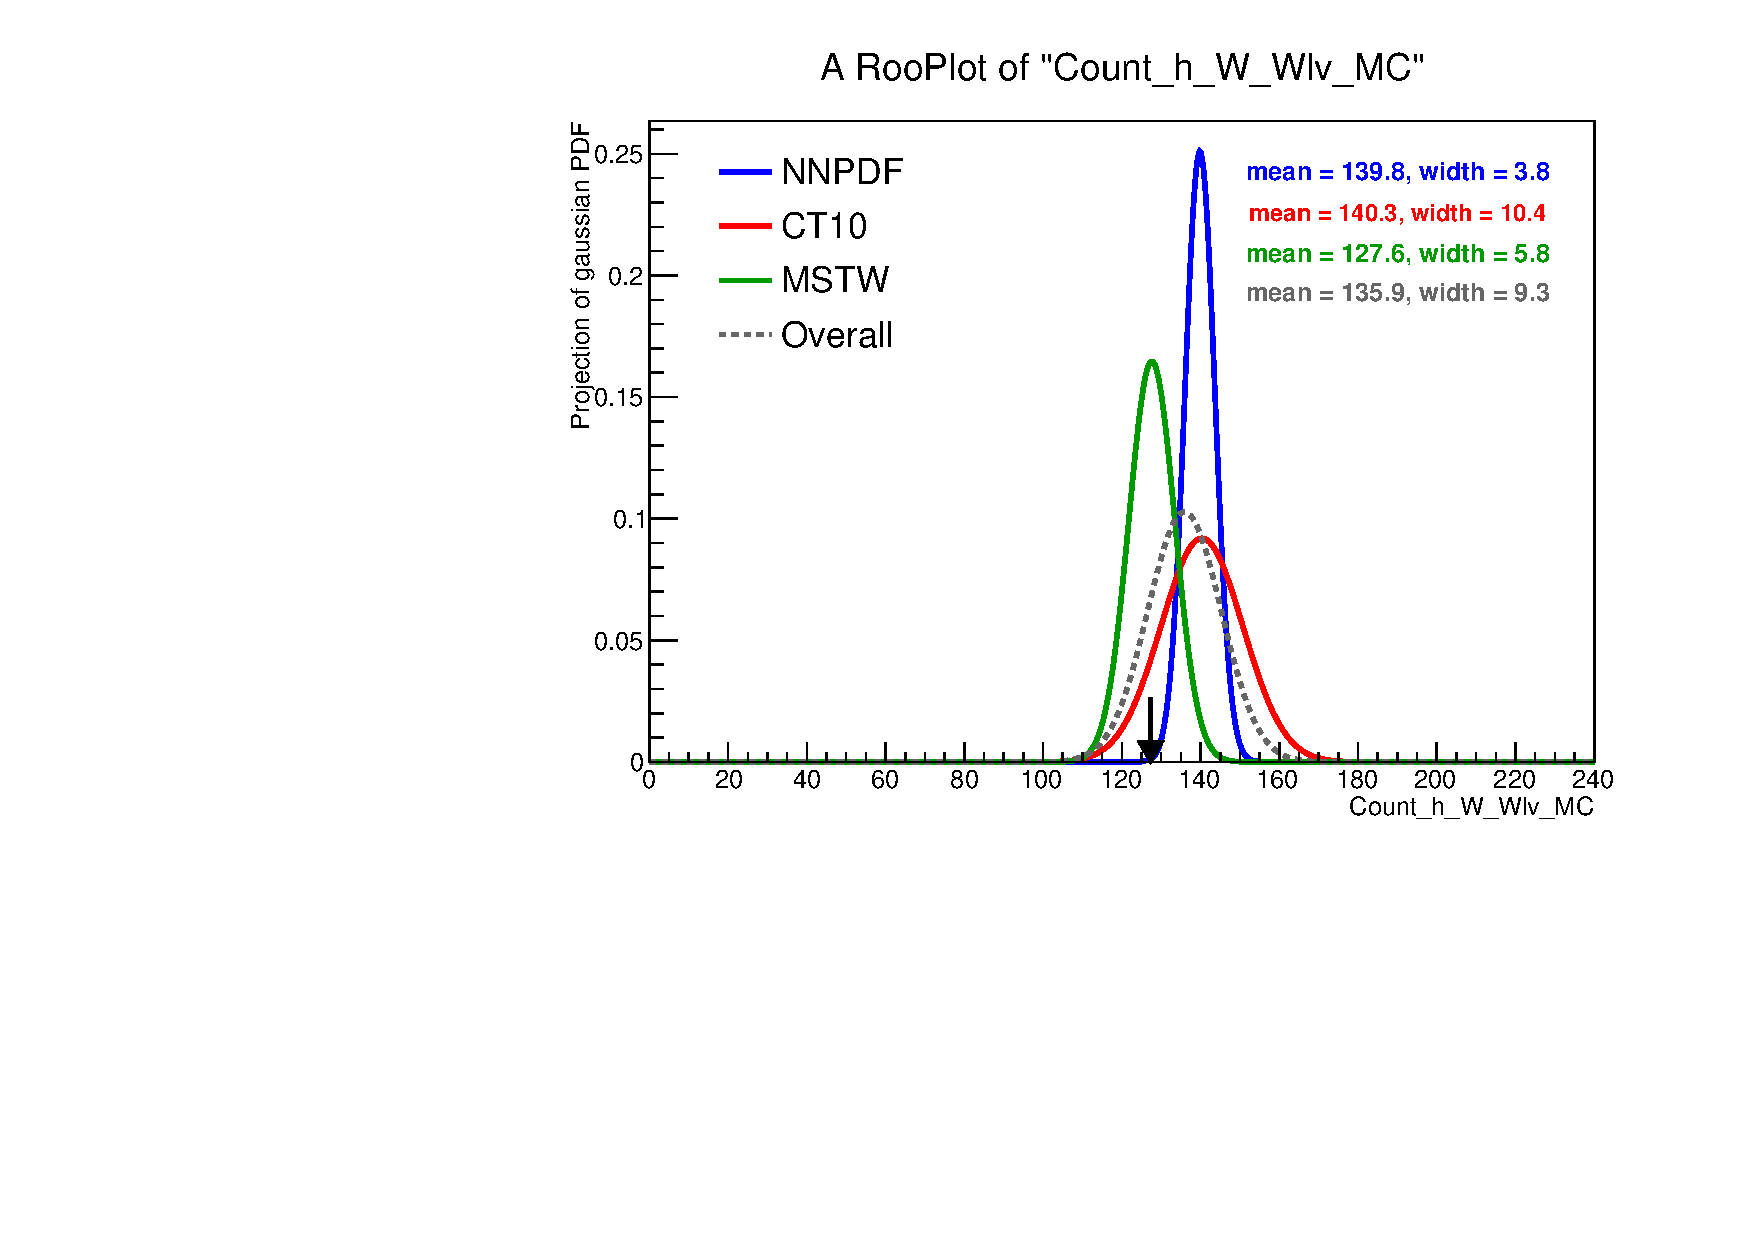
\includegraphics[width=0.49\textwidth]{figures/Systematics/PDF/h_W_Wlv_MC}
% \caption{Influence of different PDF sets on the MC counts entering $\kappa_{Wlv}^{W/S}$
% \label{fig:PDF_effect_on_bg_Wlv}}
% \end{figure}
% 
% 
% \begin{figure}[p]
% \centering
% 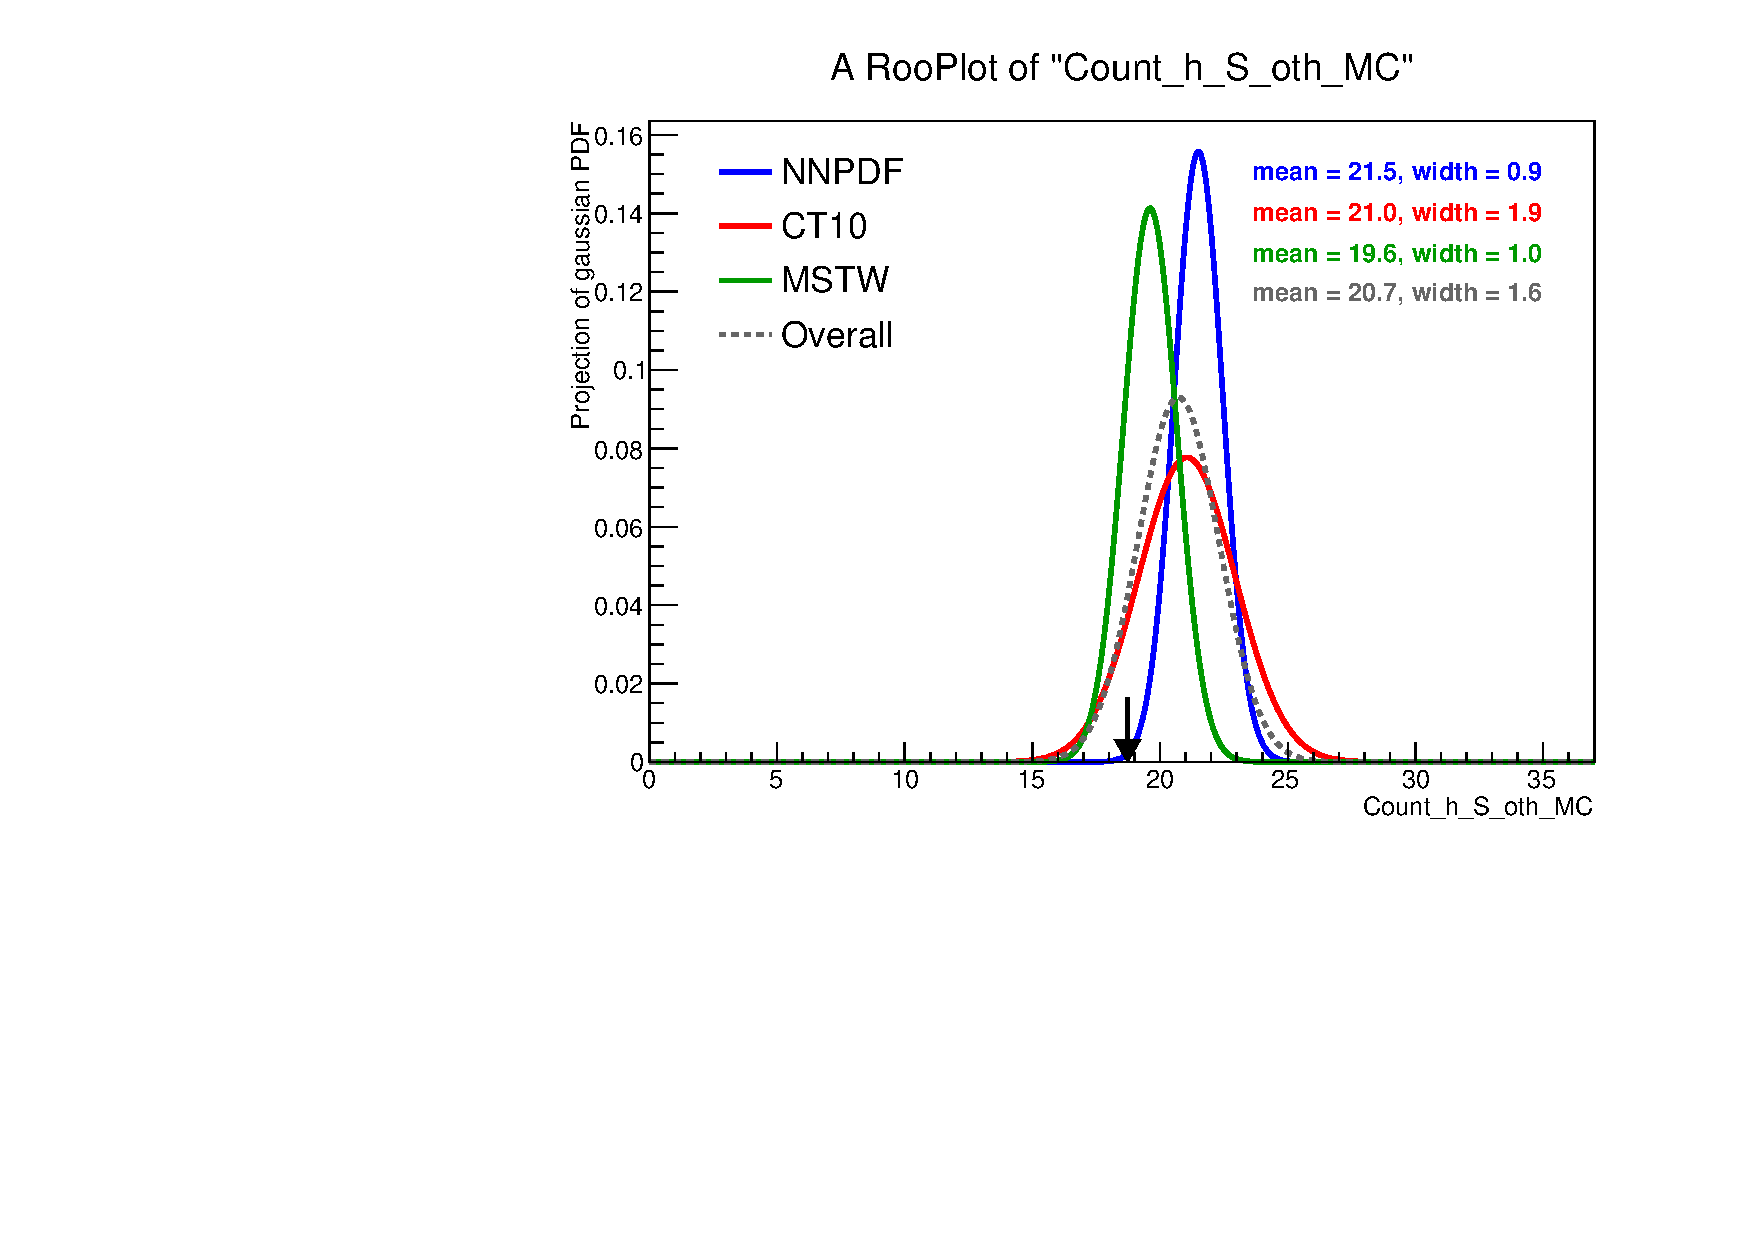
\includegraphics[width=0.49\textwidth]{figures/Systematics/PDF/h_S_oth_MC}
% 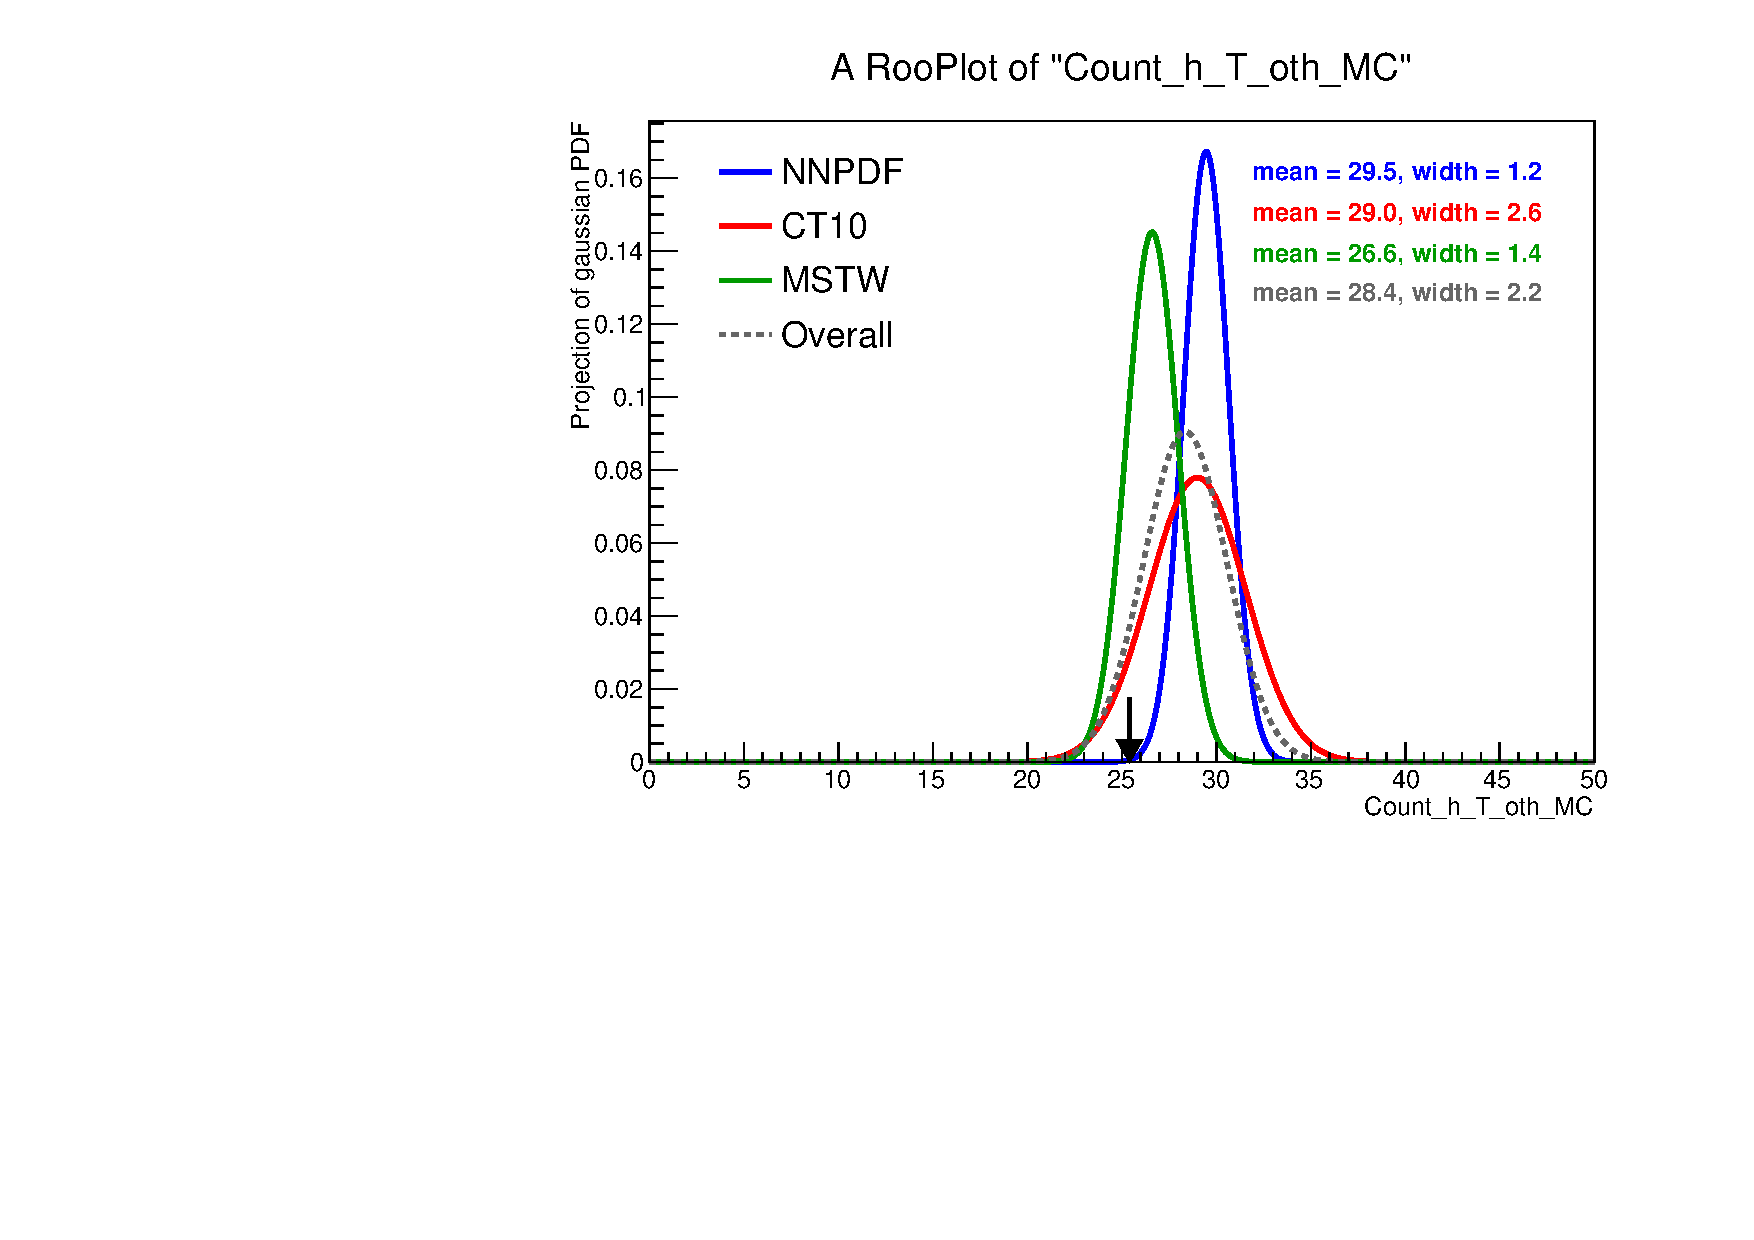
\includegraphics[width=0.49\textwidth]{figures/Systematics/PDF/h_T_oth_MC}
% \caption{Influence of different PDF sets on the MC counts in the $S$ (left) and $T$ (right) region
% for the backgrounds that are taken directly from the simulation.
% \label{fig:PDF_effect_on_bg_oth1}}
% \end{figure}
% 
% \begin{figure}[p]
% \centering
% 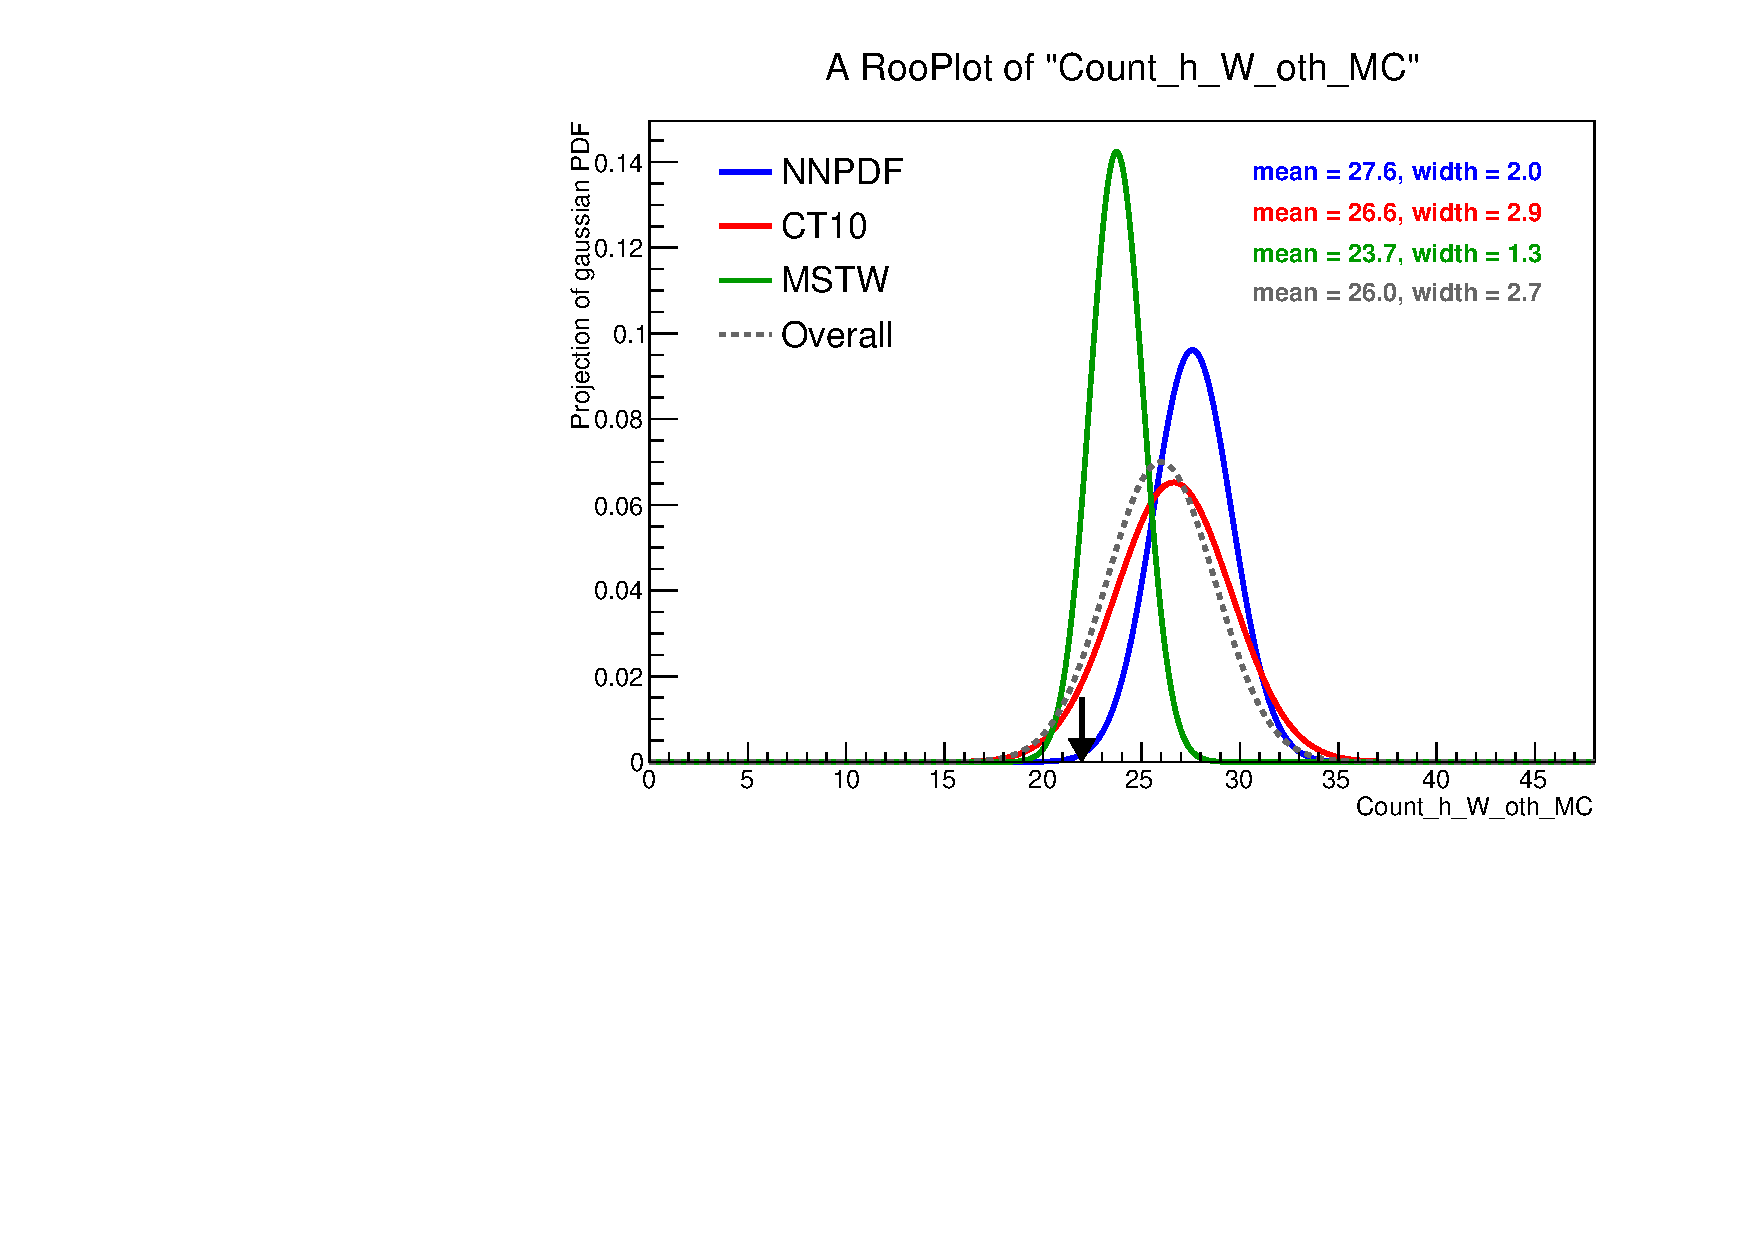
\includegraphics[width=0.49\textwidth]{figures/Systematics/PDF/h_W_oth_MC}
% 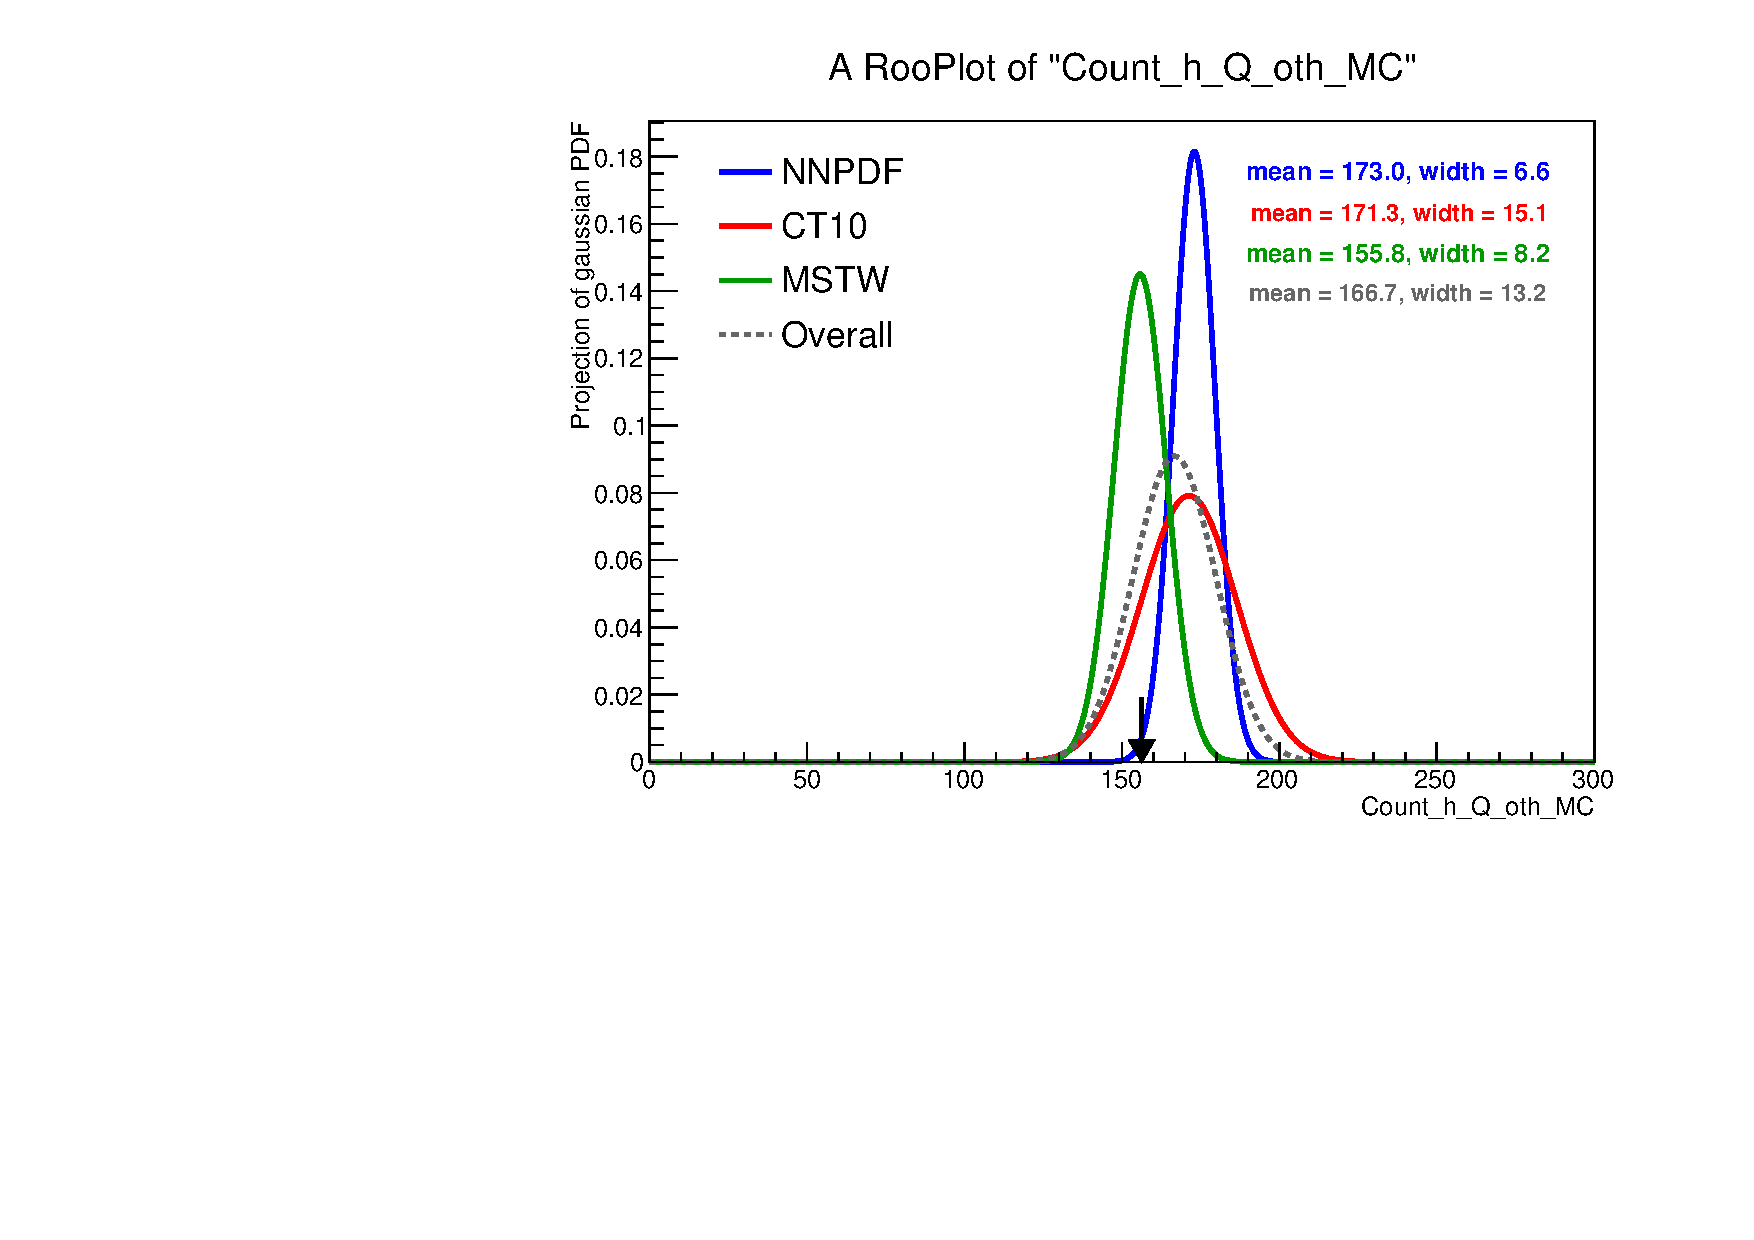
\includegraphics[width=0.49\textwidth]{figures/Systematics/PDF/h_Q_oth_MC}
% \caption{Influence of different PDF sets on the MC counts in the $W$ (left) and $Q$ (right) region
% for the backgrounds that are taken directly from the simulation.
% \label{fig:PDF_effect_on_bg_oth2}}
% \end{figure}
% 
% \begin{figure}[p]
% \centering
% 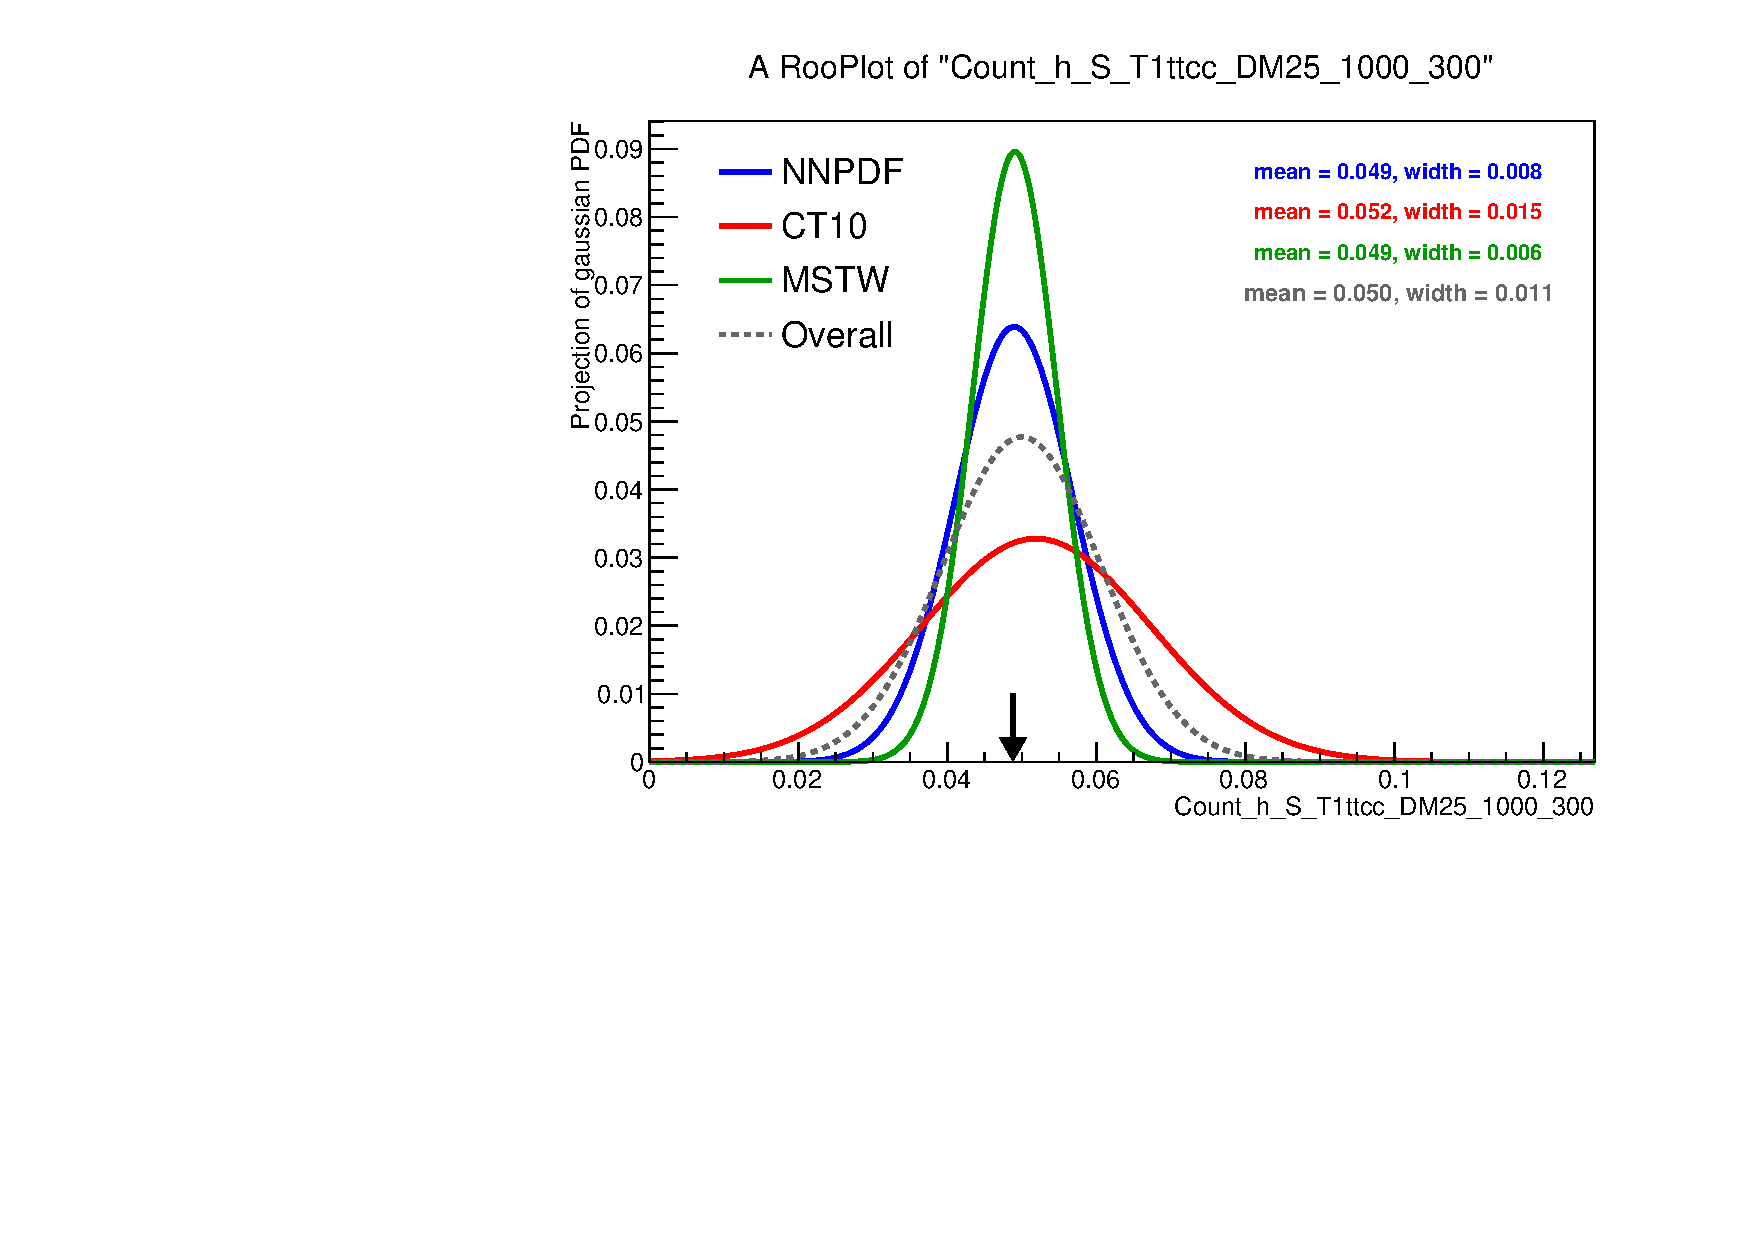
\includegraphics[width=0.7\textwidth]{figures/Systematics/PDF/h_S_T1ttcc_DM25_1000_300}
% \caption{Influence of different PDF sets on the signal efficiency for the T1ttcc signal point with
% $m_{\tilde{g}}=1000\GeV, m_{\tilde{t}_1}=325\GeV, m_{\tilde{\chi}_1^0}=300\GeV$.
% \label{fig:PDF_effect_on_sig}}
% \end{figure}
% 
% 
% %%%%%%%%%%%%%%%%%%%%%%%%%%%%%%%%%%%%%%%%%%%%%%%%%%%%%%%%%%%%%%%%%%%%%%%%%%%%%%%%%%%%%%
% 
% 
% \subsection{Trigger efficiency \label{sec:trigger_uncertainties}}
% 
% The trigger efficiency as determined in section~\ref{sec:trigger} comes with an associated
% uncertainty coming from the statistical precision of the data samples used to perform the
% measurement.   Magnitudes of the plus and minus uncertainties were shown in
% figure~\ref{fig:trigger_efficiency} as functions of $H_T$ and leading jet \pt.  We compute an event
% weight based on the efficiency and uncertainty as follows:
% \begin{eqnarray}
% w_{\rm trig} & = & \epsilon_{\rm trig}(H_T, j_1p_T) + \sigma_{\rm trig} \delta\epsilon^+_{\rm
% trig}(H_T, j_1p_T), \,\,\, {\rm if} \,\, \sigma_{\rm trig} > 0 \\ 
% w_{\rm trig} & = & \epsilon_{\rm trig}(H_T, j_1p_T) + \sigma_{\rm trig} \delta\epsilon^-_{\rm
% trig}(H_T, j_1p_T), \,\,\, {\rm if} \,\, \sigma_{\rm trig} < 0 
% \end{eqnarray}
% where $\sigma_{\rm trig}$ is a random Gaussian number.	
% 
% 
% %%%%%%%%%%%%%%%%%%%%%%%%%%%%%%%%%%%%%%%%%%%%%%%%%%%%%%%%%%%%%%%%%%%%%%%%%%%%%%%%%%%%%%
% 
% 
% \subsection[btag scale factors]{$b$-tag scale factors \label{sec:btag_uncertainties}}
% 
% Performance in $b$-tagging differs between data and simulation, and differs further between FullSim
% and FastSim.  
% To account for the differences and correct simulated events to match data, we apply data-FullSim and
% FullSim-FastSim $b$-tag scale factors (SFs), which are given as the ratios of $b$-tagging
% efficiencies, where both efficiencies and SFs are functions of jet flavor, \pt, and $\eta$.  
% 
% There are several ways to reweight events using SFs \cite{BTagSF1}.  
% Here we choose a method where we consider the number of $b$ tagged jets in an event to be fixed to
% what is given by simulation.  
% For a given event, using the $b$-tagging efficiencies for truth $b$, $c$ and $udsg$ jets with the
% relevant tagging algorithm and working point, we first compute two probabilities to have our event
% give the number of $b$ jets it has as follows: 
% we compute a $P({\rm Sim})$ using efficiencies obtained from simulated MC events, and then we obtain
% a $P(\rm data)$ using efficiencies that represent data as
% \begin{eqnarray}
% P(Sim) & = & \prod_{i={\rm tagged}} \epsilon_i^{Sim} \prod_{j={\rm not tagged}} (1 -
% \epsilon_j^{Sim}) \\
% P(Data) & = & \prod_{i={\rm tagged}} \epsilon_i^{data} \prod_{j={\rm not tagged}} (1 -
% \epsilon_j^{data})
% \end{eqnarray}
% where 
% \begin{equation}
% \epsilon^{data} = {\rm SF}^{data}_{Sim} \epsilon^{Sim} .
% \end{equation}
% Our SM MC is simulated with FullSim, so we scale the efficiency with ${\rm SF}^{data}_{Sim} = {\rm
% SF}^{data}_{Full}$.  
% However, our signal samples have been generated using FastSim, so the overall scale factor becomes
% ${\rm SF}^{data}_{Sim} = {\rm SF}^{data}_{Full} {\rm SF}^{Full}_{Fast}$.
% The ratio of the two probabilities, $w = P(Data) / P(Sim)$, gives us the weight to scale the event.
%  
% The input efficiencies $\epsilon_j^{\rm Sim}$ are previously obtained from MC events.  
% 
% We take into account the uncertainties on the SFs as systematics.  
% To do this, we sample $n$ numbers $\sigma$ from a Gaussian with mean 0 and sigma 1 (we sample
% different $\sigma$s for FullSim and FastSim, and also for different jet truth flavors).  
% We then run our analysis $n$ times, where each time we use given $\sigma$s to compute
% $\epsilon^{data}$ as follows:
% \begin{eqnarray}
% \epsilon^{data} & = & ({\rm SF}^{data}_{Full} + \sigma_1 \, \delta {\rm SF}^{data}_{Full} )
% \epsilon^{Full} \\
% \epsilon^{data} & = & ({\rm SF}^{data}_{Full} + \sigma_1 \, \delta {\rm SF}^{data}_{Full} )({\rm
% SF}^{Full}_{Fast} + \sigma_2 \, \delta {\rm SF}^{Full}_{Fast} ) \epsilon^{Fast}.
% \end{eqnarray}
% For each of the $n$ runs, different $\epsilon^{data}$s will lead to different weights $w$ for a
% given event, and overall, the weighted yields will differ.  We obtain the systematic from the
% ensemble of the resulting $n$ yields.
% 
% In this study, we use CSVM and CSVL taggers, which are always used independent of each other.  
% Therefore, for a given event, we compute separate weights $w$ with CSVM and CSVL, and implement them
% in the relevant regions (e.g., we use the CSVM weight in the signal region and CSVL weight in the
% QCD region).
% 
% 
% %%%%%%%%%%%%%%%%%%%%%%%%%%%%%%%%%%%%%%%%%%%%%%%%%%%%%%%%%%%%%%%%%%%%%%%%%%%%%%%%%%%%%%
% 
% 
% \subsection[W tag scale factors]{$\PW$ tag scale factors \label{sec:Wtag_SF}}
% 
% 
% 
% %%%%%%%%%%%%%%%%%%%%%%%%%%%%%%%%%%%%%%%%%%%%%%%%%%%%%%%%%%%%%%%%%%%%%%%%%%%%%%%%%%%%%%
% 
% 
% \subsection{Lepton ID}
% 
% Our analysis requires a single loose lepton in the definitions of top and $W$ control regions.  We
% therefore apply lepton scale factors to our events and incorporate the lepton scale factor
% uncertainty as a systematic.  For electrons, we use the $p_T$ and $\eta$-dependent scale factors and
% uncertainties derived by the Egamma POG, which could be found in:
% {\small
% \begin{verbatim}
% https://twiki.cern.ch/twiki/bin/view/Main
%       /EGammaScaleFactors2012#2012_8_TeV_Jan22_Re_recoed_data
% \end{verbatim}}
% 
% The overall event weight is given as:
% \begin{equation}
% w_{eL} = {\rm SF_{eL}}(p_T, \eta) + \sigma_{\rm eL} \delta {\rm SF_{eL}}(p_T, \eta)
% \end{equation}
% where $\sigma_{\rm eL}$ is a random Gaussian number.
% 
% We ignore the scale factors and uncertainties for muons, since the scale factors are approximately 1
% and the uncertainties are negligible.
% 
% 
% %%%%%%%%%%%%%%%%%%%%%%%%%%%%%%%%%%%%%%%%%%%%%%%%%%%%%%%%%%%%%%%%%%%%%%%%%%%%%%%%%%%%%%
% 
% 
% \subsection{ISR reweighting}
% 
% For the signal samples the recommendation is to apply the so-called ISR reweighting recipe. The
% details were explained in section~\ref{sec:ISRreweighting}. 
% The size of the associated systematic uncertainty depends on the \pt of the recoiling system, and is
% equal to the difference $1 - w_{ISR}$, where $w_{ISR}$ is the weight associated to the ISR
% reweighting. 
% The one sigma up variation is thus always consistent with no reweighting. 
% 
% 
% %%%%%%%%%%%%%%%%%%%%%%%%%%%%%%%%%%%%%%%%%%%%%%%%%%%%%%%%%%%%%%%%%%%%%%%%%%%%%%%%%%%%%%
% 
% 
% \subsection{Top pT reweighting}
% 
% For more details on the top \pt reweighting recipe, we refer to
% section~\ref{sec:toppt_reweighting}. 
% The uncertainties associated with this reweighting are defined as follows:
% the one sigma down variation corresponds to no reweighting at all;
% the one sigma up variation corresponds to applying the reweighting twice. 
% 
% These uncertainties are propagated to the Data/MC ratio used in the estimation of the TTjets
% background. 
% 
% 
% %%%%%%%%%%%%%%%%%%%%%%%%%%%%%%%%%%%%%%%%%%%%%%%%%%%%%%%%%%%%%%%%%%%%%%%%%%%%%%%%%%%%%%
% 
% 
% \subsection{PU reweighting}
% 
% In order to account for uncertainties related to the PU reweighting, it is recommended to derive the
% up/down weights by varying the minbias cross section by +-5\%. This will result in a different shape
% for the data pileup, and thus in a different set of weights. 
% The difference in weights is used as the sigma of a gaussian from which we sample when doing the
% simultaneous sampling of all systematic uncertainties. 
% 
% %%%%%%%%%%%%%%%%%%%%%%%%%%%%%%%%%%%%%%%%%%%%%%%%%%%%%%%%%%%%%%%%%%%%%%%%%%%%%%%%%%%%%%
% 
% 
% \subsection{Shape systematics affecting the MC translation factors \label{sec:shape_systematics}}
% 
% In order to assess additional systematics related to the MC translation factors, we can use the two
% closure tests we explained in section~\ref{sec:Shape_sideband} and \ref{sec:Shape_QCD}. The level of
% closure in these tests can be used to derive an additional systematic uncertainty if it turns out
% that the closure is not covered by the sizeable statistical uncertainty and the other systematic
% uncertainties already considered.
% 
% To make it easier to use the results of the closure tests, we provide the results of the closure
% tests in a different format. Figures~\ref{fig:closure_green} and \ref{fig:closure_magenta} show each
% bin (containing data/prediction) in the 2D $M_R - R^2$ plane plotted next to each other, starting
% with the first $R^2$ strip for fixed $M_R$ and then moving along to the next strip for the next
% $M_R$ value. 
% 
% \begin{figure}[htpb]
% \centering
% \includegraphics[width=0.7\textwidth]{figures/ShapeSyst/closure_summary_0p5_green}
% \caption{Data/Prediction for each bin in the 2D $M_R-R^2$ plane for the closure test predicting the
% $\Delta\phi_{min}$ sideband of the S region. Uncertainties are statistical only.
% \label{fig:closure_green}}
% \end{figure}
% 
% \begin{figure}[htpb]
% \centering
% 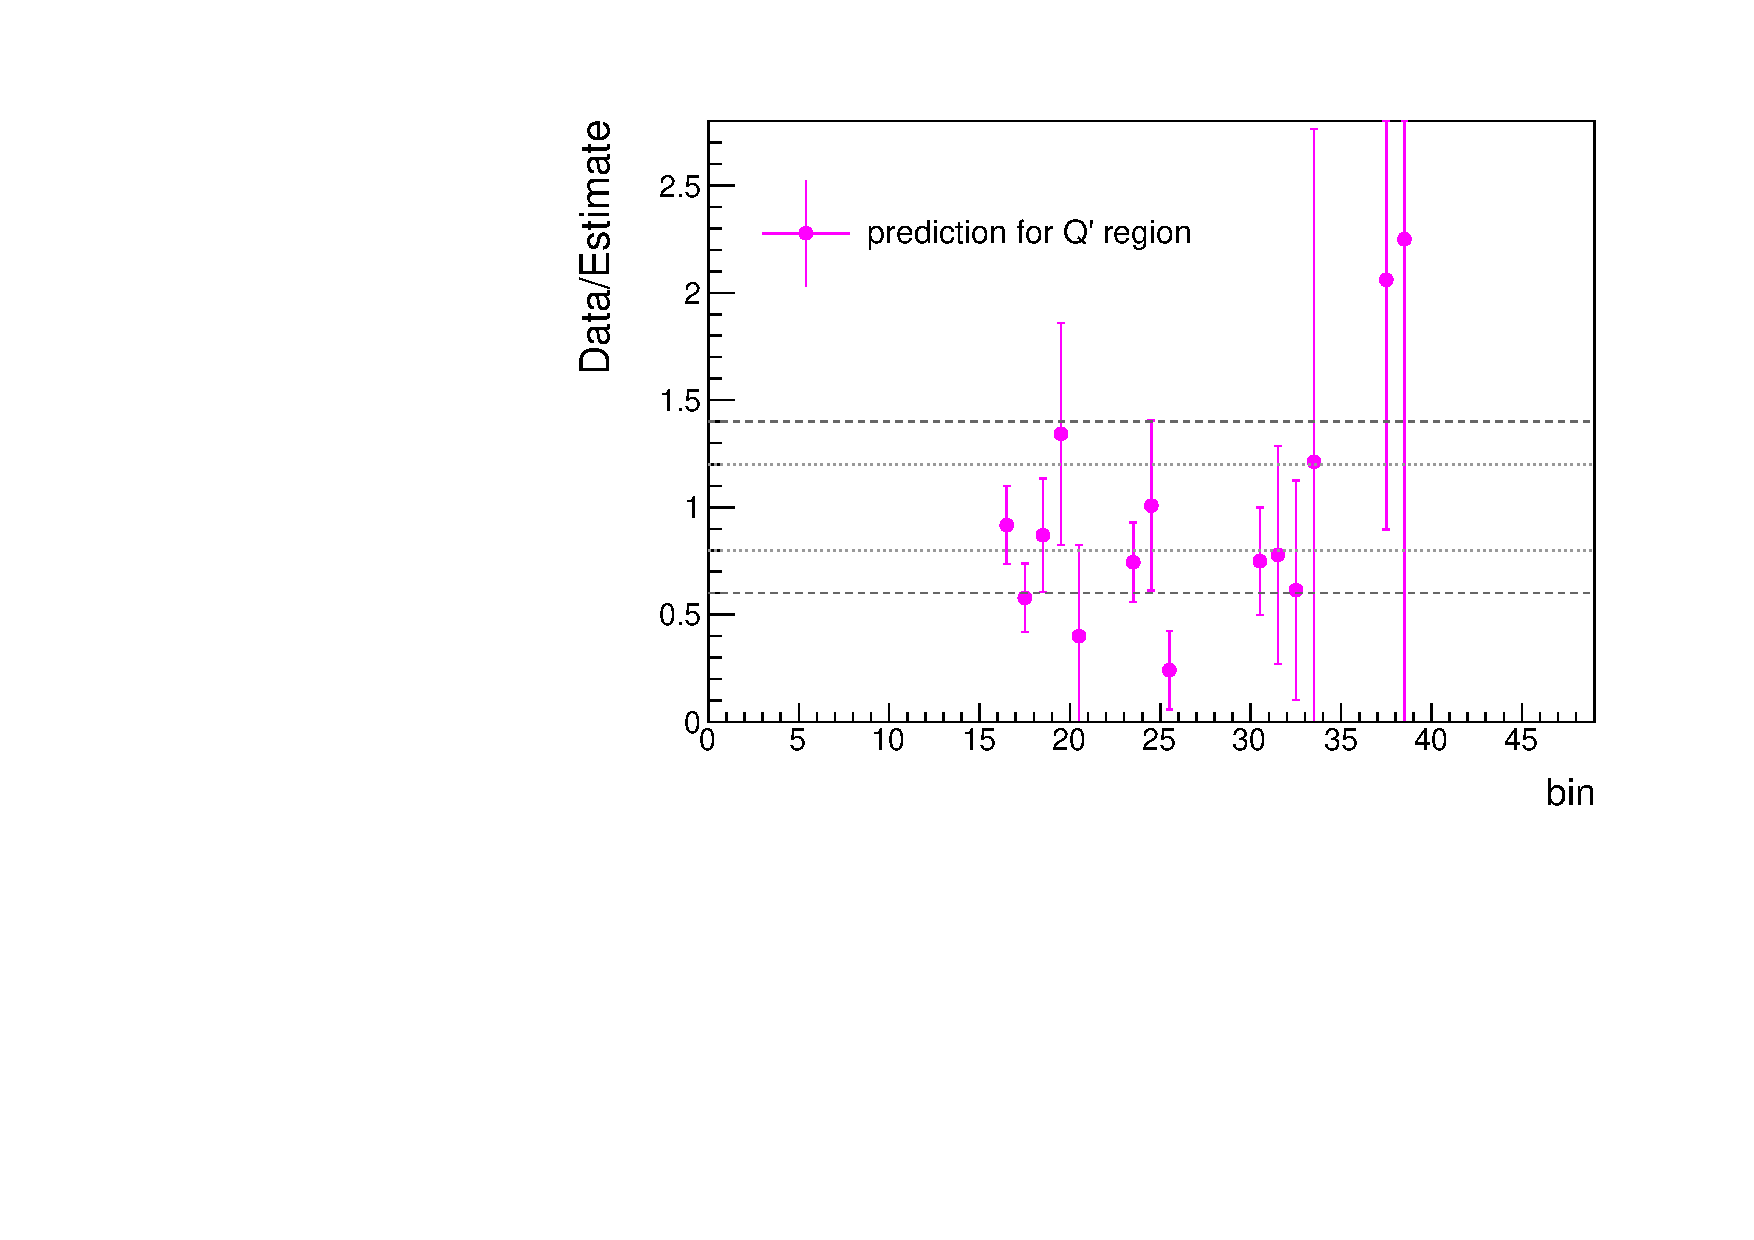
\includegraphics[width=0.7\textwidth]{figures/ShapeSyst/closure_summary_0p5_magenta}
% \caption{Data/Prediction for each bin in the 2D $M_R-R^2$ plane for the closure test predicting the
% high $\Delta\phi_{min}$ region of the Q control region. Uncertainties are statistical only.
% \label{fig:closure_magenta}}
% \end{figure}
% 
% Using the ratios between observed data and the prediction from the closure tests, we can derive a
% systematic uncertainty that we can apply on the MC ratios we use in the actual background
% estimation. 
% To do this we model each bin in the 2D plane as a Gaussian, taking the uncertainty in that bin as
% the width of the Gaussian, weight them with $\sqrt{N_{obs}}$ to give more weight to bins with higher
% precision and add all of them up. 
% From the summed distribution we can then compute the interval around 1 that contains approximately
% 68\% of the integral. 
% 
% The results of this procedure are shown in Figure~\ref{fig:closure_green_gauss} for the first
% closure test, and in Figure~\ref{fig:closure_magenta_gauss} for the second closure test. 
% 
% The 68\% range for the first closure test corresponds to a $\pm 20\%$ range, while for the second
% closure test it corresponds to $\pm 40\%$.
% These systematics are summarized in table~\ref{tab:shape_syst} for each considered MC ratio,
% $\kappa$.
% 
% As the total uncertainty on $\kappa_{QCD}^{Q/S}$ without including this closure test, is of the
% order of 25\%, we will inflate this uncertainty to 40\%, to cover for the shape difference observed
% in closure test two. 
% The observed uncertainty on the other $\kappa$'s is already sufficient. 
% 
% \begin{table}[htpb]
% \renewcommand*{\arraystretch}{1.4}
% \centering
% \caption{Summary of shape systematics \label{tab:shape_syst}}
% \begin{tabular}{|c|c|c|}
% \hline
% Translation factor & Closure test 1 & Closure test 2 \\
% \hline
% $\kappa_{TTJ}^{T/S}$ & 20\% & - \\
% $\kappa_{WJ}^{W/S}$  & 20\% & -  \\
% $\kappa_{QCD}^{Q/S}$ & 20\% & 40\%  \\
% $\kappa_{QCD}^{T/Q}$ & 20\% & 40\%  \\
% \hline
% \end{tabular}
% \end{table}
% 
% \begin{figure}[htpb]
% \centering
% \includegraphics[width=0.49\textwidth]{figures/ShapeSyst/closure_summary_0p5_green_gauss}
% \includegraphics[width=0.49\textwidth]{figures/ShapeSyst/closure_summary_0p5_green_gauss2}
% \caption{[left] We represent the agreement between data and prediction for the closure test
% predicting the $\Delta\phi_{min}$ sideband of the S region as a Gaussian pdf for each bin in the 2D
% $M_R-R^2$ plane. Each bin is shown as a normalized gaussian in a different shade of magenta. The sum
% of all Gaussians is depicted in black. 
% [right] Same as on left plot, but each separate component is now normalized to the weight it carries
% in the sum. 
% \label{fig:closure_green_gauss}}
% \end{figure}
% 
% \begin{figure}[htpb]
% \centering
% \includegraphics[width=0.49\textwidth]{figures/ShapeSyst/closure_summary_0p5_magenta_gauss}
% 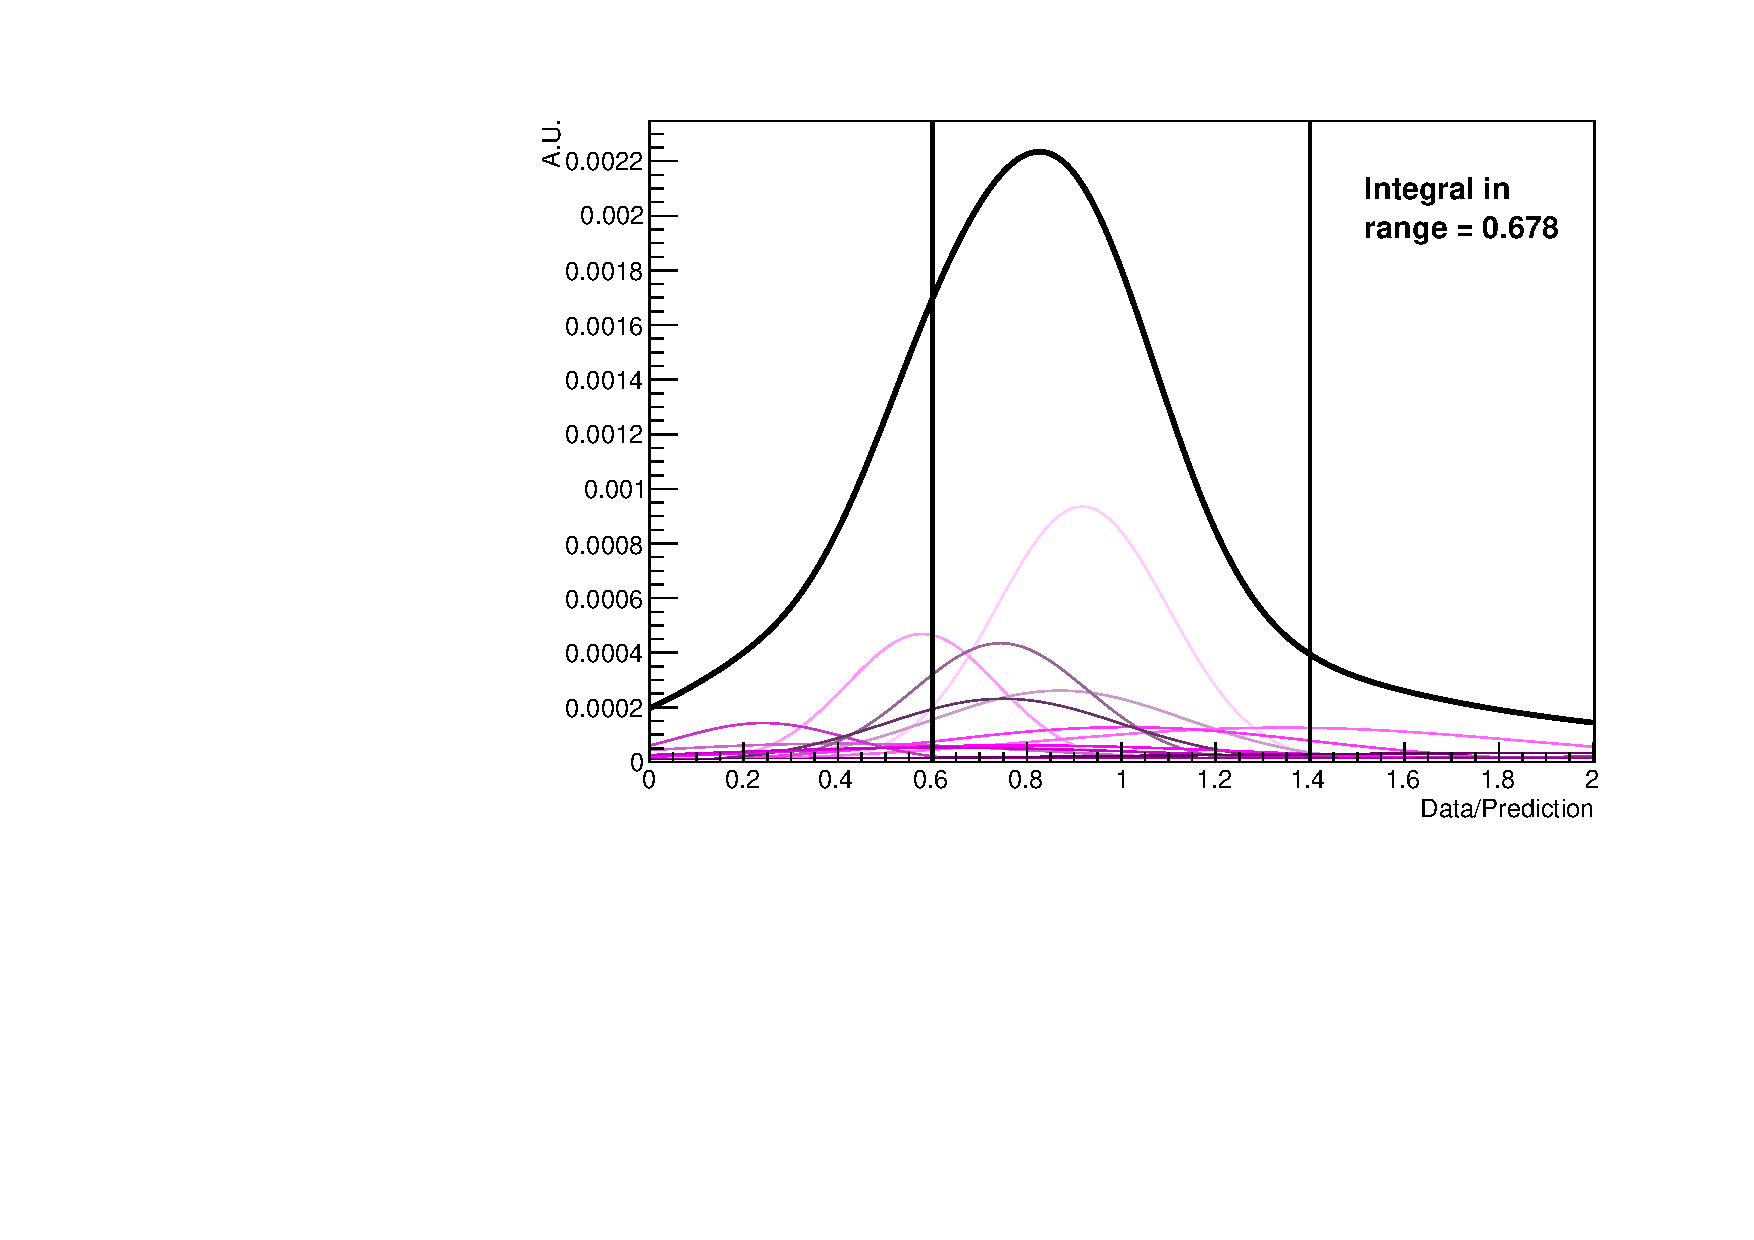
\includegraphics[width=0.49\textwidth]{figures/ShapeSyst/closure_summary_0p5_magenta_gauss2}
% \caption{[left] We represent the agreement between data and prediction for the closure test
% predicting the high $\Delta\phi_{min}$ region of the Q control region as a Gaussian pdf for each bin
% in the 2D $M_R-R^2$ plane. Each bin is shown as a normalized gaussian in a different shade of
% magenta. The sum of all Gaussians is depicted in black. 
% [right] Same as on left plot, but each separate component is now normalized to the weight it carries
% in the sum. 
% \label{fig:closure_magenta_gauss}}
% \end{figure}
% 
% 
% %%%%%%%%%%%%%%%%%%%%%%%%%%%%%%%%%%%%%%%%%%%%%%%%%%%%%%%%%%%%%%%%%%%%%%%%%%%%%%%%%%%%%%
% 
% 
% \subsection[Uncertainty on Znunu modeling]{Uncertainty on $Z\rightarrow\nu\nu$ modeling}
% 
% About 7-8\% of the background in our signal region is composed of $Z\rightarrow\nu\nu$+jets. As we
% are requiring the presence of at least one $b$-tagged jet, and we know that $Z$ production in
% association with heavy flavour is not well modeled, we need to apply an extra systematic uncertainty
% on the $Z\rightarrow\nu\nu$ +jets contribution. 
% 
% To derive this uncertainty, we define a control region in data, enriched in $Z\rightarrow l
% \bar{l}$, and as close as possible to the signal region. 
% The selection applied to this control region is: 
% \begin{itemize}
% \item at least one good vertex
% \item at least three jets
% \item $\pt(\textrm{jet}_1) > 200\GeV$
% \item $M_R > 800\GeV$ and $R^2 > 0.08$
% \item exactly two tight leptons, same flavour and opposite sign ($e$ or $\mu$)
% \item $60 < m_{ll} < 120$
% \item at least one $b$-tagged jet
% \item at least one $Y$ (mass-tagged jet)
% \end{itemize}  
% 
% Figure~\ref{fig:DataMC_ZCR} shows the Data/MC comparison for $M_R$ and $R^2$. 
% To derive an uncertainty using this comparison, we use the same procedure as explained in
% section~\ref{sec:shape_systematics}. 
% The results are shown in Figure~\ref{fig:1D_ZCR} and \ref{fig:ZCR_syst}. 
% Based on these results, we decide to put an additional uncertainty on the $Z\rightarrow\nu\nu$ cross
% section of 50\%. 
% 
% \begin{figure}[htpb]
% \centering
% 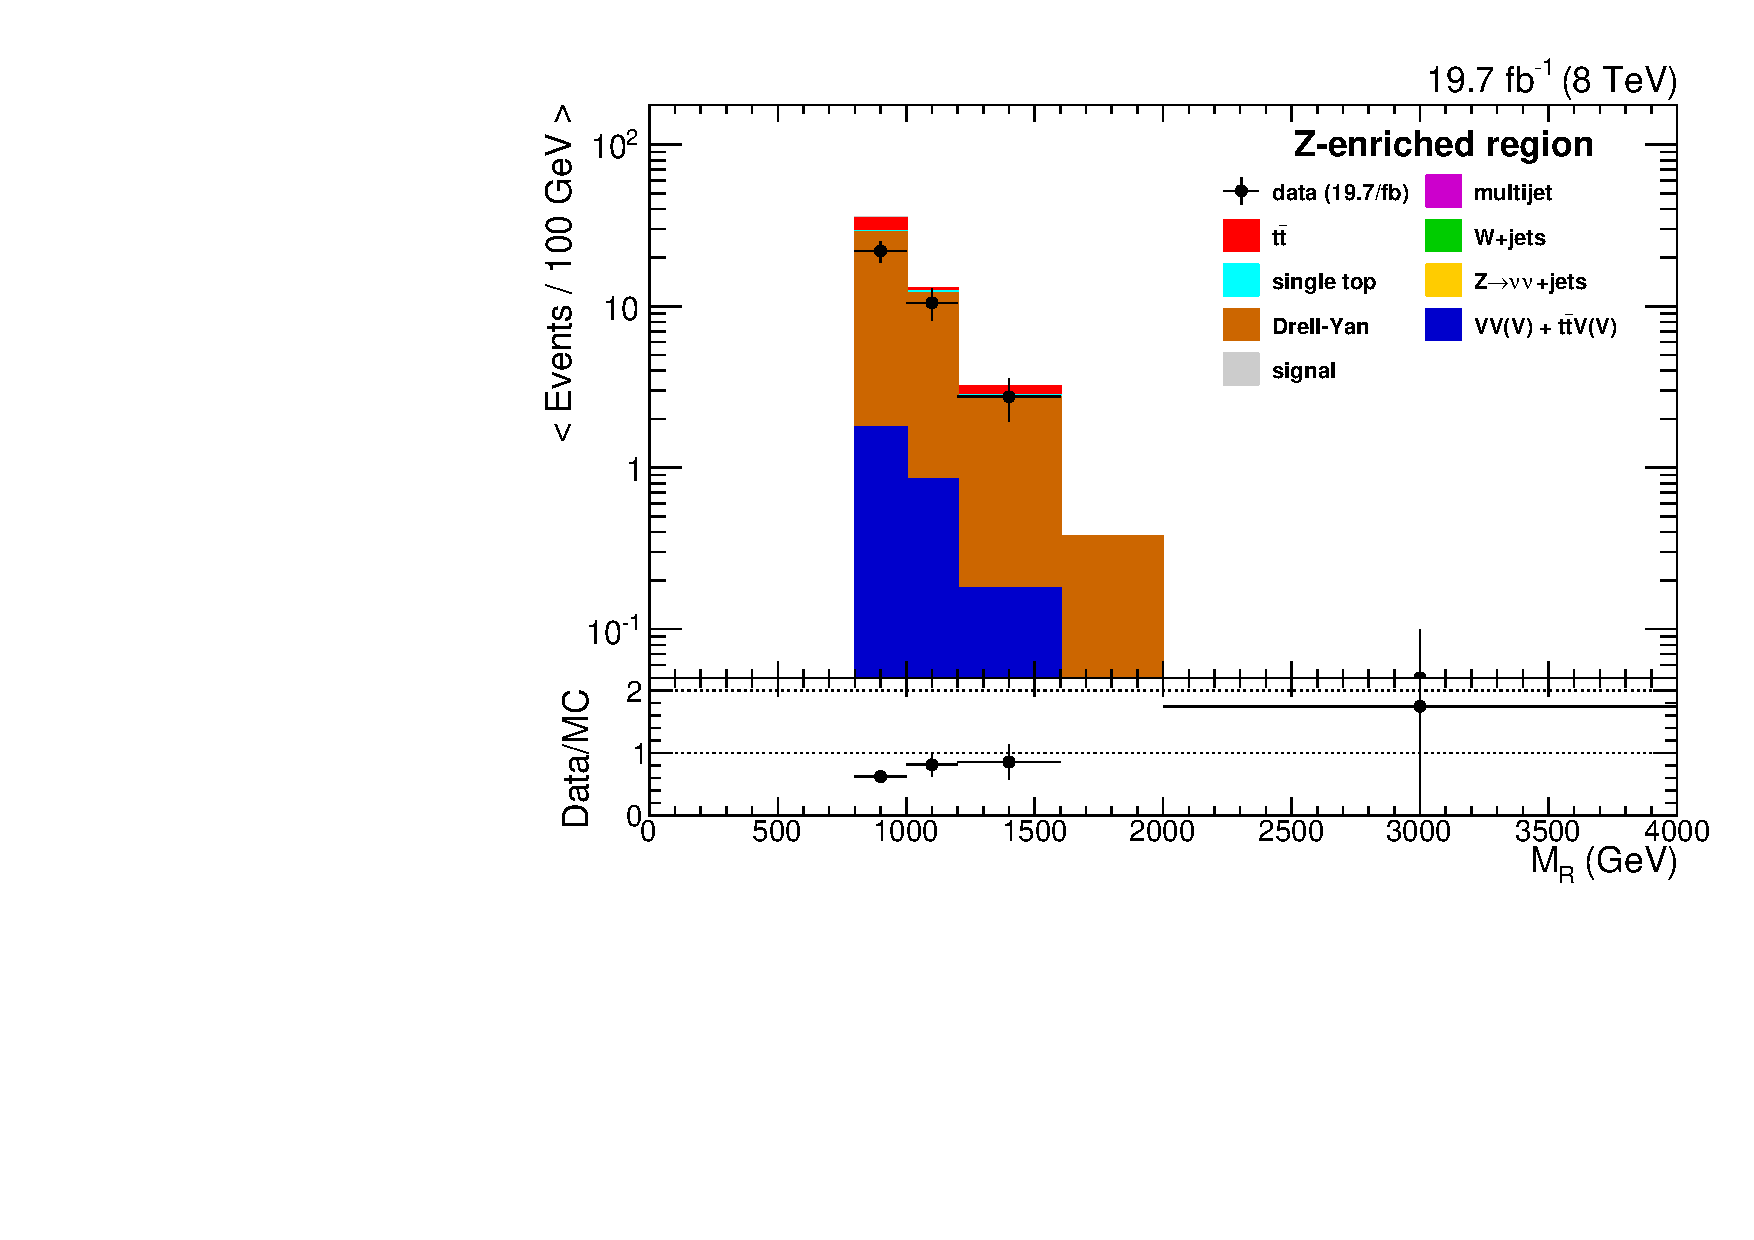
\includegraphics[width=0.49\textwidth]{figures/DataMC/DataMC_MR_g1Mbg1Y2l0ol_width}
% 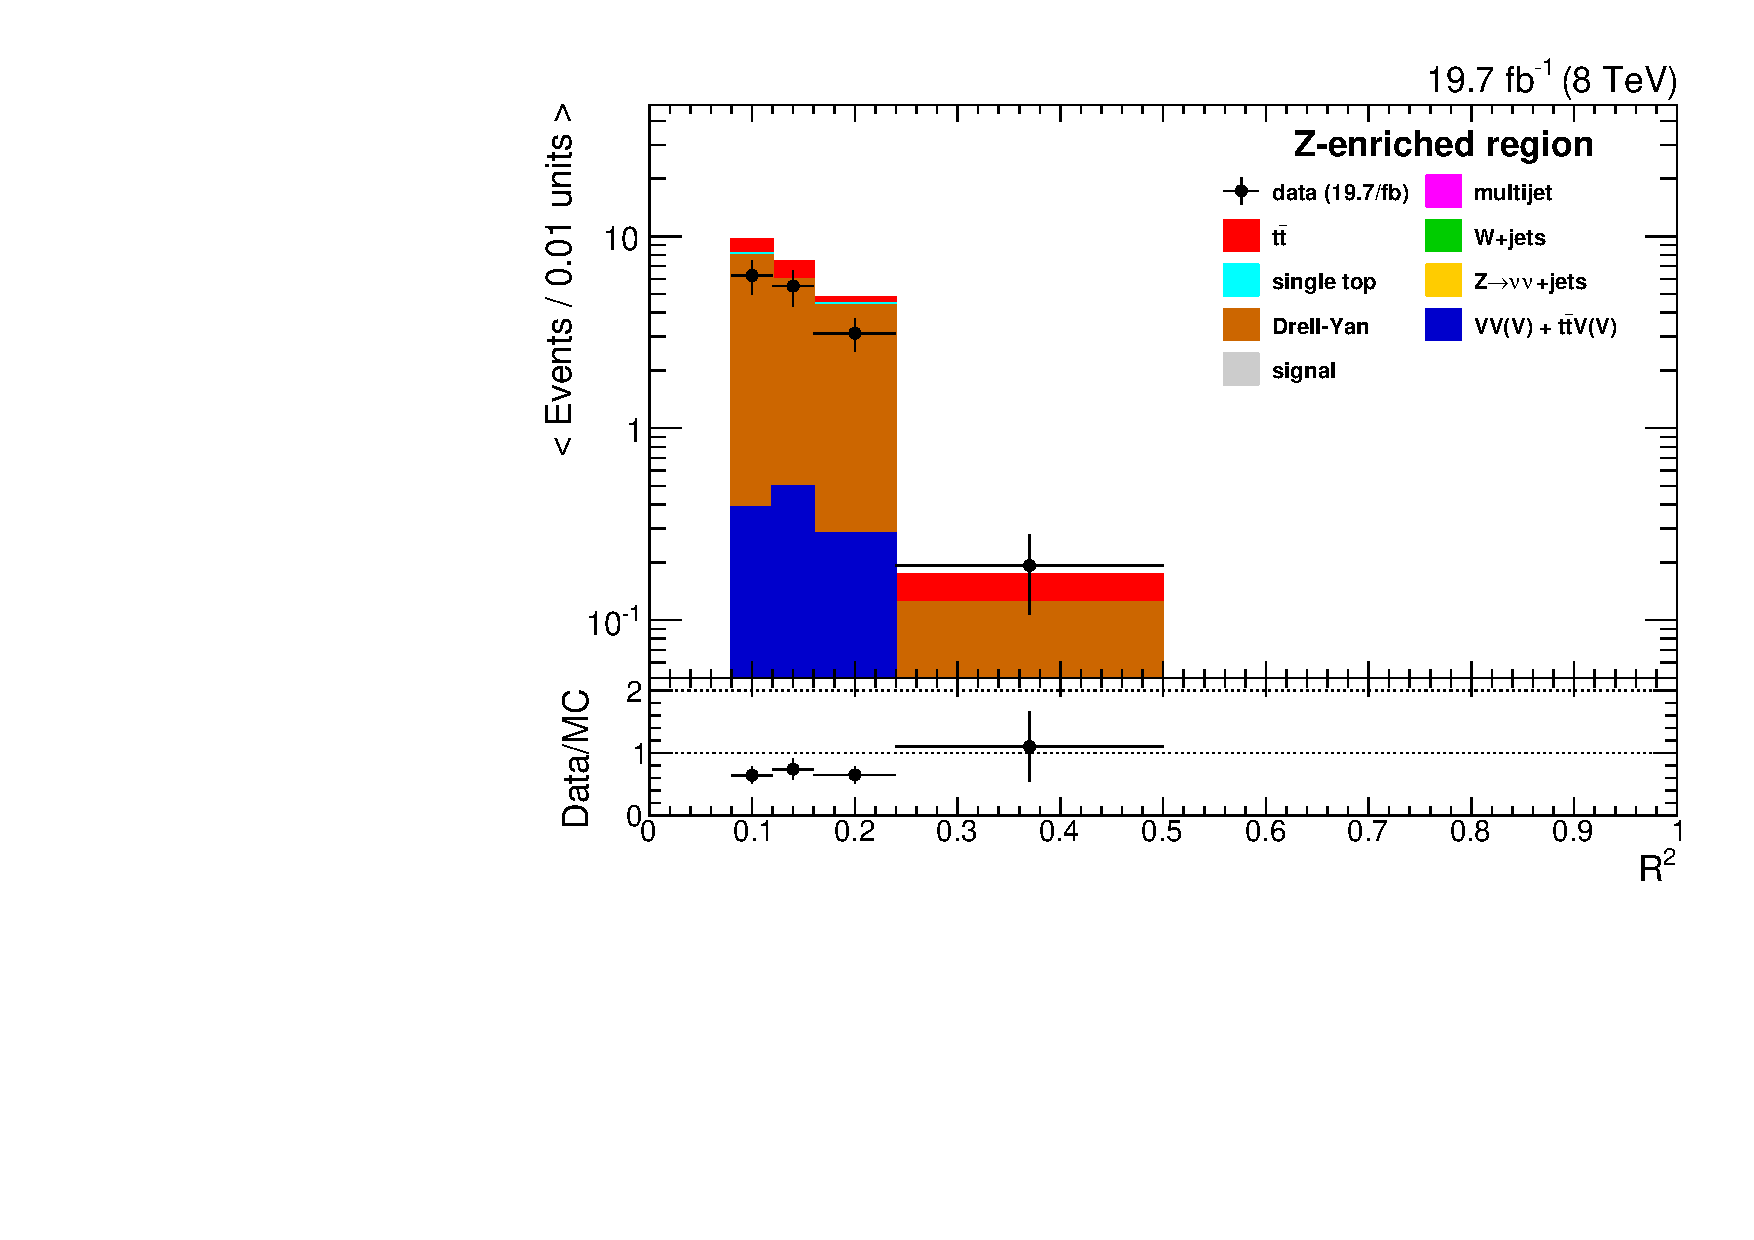
\includegraphics[width=0.49\textwidth]{figures/DataMC/DataMC_R2_g1Mbg1Y2l0ol_width}
% \caption{Data/MC comparison for $M_R$ (left) and $R^2$ (right) in the $Z\rightarrow l \bar{l}$
% control region with at least one $b$-jet and at least one mass-tagged $W$-candidate. 
% \label{fig:DataMC_ZCR}}
% \end{figure}
% 
% \begin{figure}[htpb]
% \centering
% \includegraphics[width=0.7\textwidth]{figures/Zinv_DataMC_1D}
% \caption{Data/Simulation for each bin in the 2D $M_R-R^2$ plane for the $Z\rightarrow l \bar{l}$
% control region. Uncertainties are statistical only.
% \label{fig:1D_ZCR}}
% \end{figure}
% 
% \begin{figure}[htpb]
% \centering
% \includegraphics[width=0.49\textwidth]{figures/Zinv}
% \includegraphics[width=0.49\textwidth]{figures/Zinv2}
% \caption{[left] We represent the agreement between data and simulation for the $Z\rightarrow l
% \bar{l}$ control region as a Gaussian pdf for each bin in the 2D $M_R-R^2$ plane. Each bin is shown
% as a normalized gaussian in a different shade of magenta. The sum of all Gaussians is depicted in
% black. 
% [right] Same as on left plot, but each separate component is now normalized to the weight it carries
% in the sum. 
% \label{fig:ZCR_syst}}
% \end{figure}
% 
% 
% %%%%%%%%%%%%%%%%%%%%%%%%%%%%%%%%%%%%%%%%%%%%%%%%%%%%%%%%%%%%%%%%%%%%%%%%%%%%%%%%%%%%%%
% 
% 
% \subsection{Signal systematic uncertainties results \label{sec:signal_systematics}}
% 
% As explained before, we vary all systematics simultaneously, thus sampling the systematic parameter
% space in a coherent way, taking care of all correlations. 
% To get a sense of the magnitude of each individual systematic, we also varied them $1\sigma$ up and
% down. The results of this are reported in table~\ref{tab:signal_systematics}. We give the average
% value over all mass points in the T1ttcc DM25 plane, as well as the minimum and maximum variation
% found. 
% For the PDF systematics, we ran over 100 different PDF set members (as explained in
% section~\ref{sec:PDFweights}) and fitted a gaussian to the signal efficiency distribution. The width
% of that Gaussian is taken as the size of the systematic effect. 
% The last line in the table corresponds to the full systematics sampling. To obtain this value we
% again fit a gaussian to the signal efficiency distrubution obtained from the systematic sampling. In
% Appendix~\ref{app:signal_systematics} we show the effect of each systematic on the 2D SMS plane. 
% 
% As is visible from the above mentioned plots and table, the main source of systematic uncertainty
% for the signal is the uncertainty on the parton distribution functions. The uncertainty is 15-25\%
% depending on the mass point. 
% The second leading source is the uncertainty on the W tagging scale factor for FullSim, which is
% about 9\%. 
% Finally, for very compressed mass points, the uncertainty on the ISR modeling reached about 20\%,
% compared to 4-7\% for non-compressed spectra. 
% 
% {
%\renewcommand{\arraystretch}{1.4}
\begin{table}[htpb]
\centering
\caption{Summary of $\pm 1 \sigma$ systematic uncertainties for the average signal count of all {\it T1ttcc} ($\Delta m=25\GeV$) signal points, and for the total background count in the signal region, unless indicated otherwise, as determined from simulation.  \label{tab:bgsigsys}}
\vspace{1ex}
\begin{tabular}{l c c}
\toprule
Systematic Effect & Signal up down & Background up down \\
\midrule
JEC & $ +2.2\% -2.1\%$   & $ +10.9\% -5.2\%$\\ 
Trigger & $ +1.1\% -3.3\%$ & $ +3.4\% -5.7\%$\\
b tag FullSim & $ +2.1\% -2.3\%$& $+3.9\% -4.0\%$\\
b tag FastSim & $ +1.2\% -1.3\%$& - \\
W tag efficiency Fullsim & $ +9.0\% -8.9\%$& $+4.6\% -4.6\%$\\
W tag efficiency FastSim & $ +2.2\% -2.2\%$& - \\
W tag fake rate FullSim & - & $ +1.4\% -1.4\%$ \\
W anti-tag fake rate FullSim ($Q$ region only) & - & $+2.6\% -2.6\%$ \\ 
W mass-tag fake rate FullSim ($W$ region only) & - & $+2.3\% -2.3\%$ \\ 
Electron ID ($T$ and $W$ region only) & - & $+0.2\% -0.2\%$ \\ 
Pileup & $ +0.5\% -0.5\%$ & $+1.0\% -1.1\%$\\
ISR & $ +6.6\% -6.6\%$ & - \\
Top \pt spectrum & - & $ -14.4\% ~ 20.5\%$ \\
$\cPZ\rightarrow\nu\nu+$ heavy flavour  & - & $+4.0\% -4.0\%$ \\
PDF & $20.7\%$ &  $10.7\%$ \\
\midrule
All &  $24.4\%$ &  $22.1\%$ \\
\bottomrule
\end{tabular}
\end{table}
}
 
% 
% 
% %%%%%%%%%%%%%%%%%%%%%%%%%%%%%%%%%%%%%%%%%%%%%%%%%%%%%%%%%%%%%%%%%%%%%%%%%%%%%%%%%%%%%%
% 
% 
% \subsection{Background systematic uncertainties results \label{sec:background_systematics}}
% 
% To get a sense of the background systematic effects, we provide the $\pm 1\sigma$ variations for the
% separate systematic uncertainties for several MC event counts. 
% In table~\ref{tab:bg_systematics_S_tot} we show the systematic uncertainties on the total event
% count in the signal region. 
% This count is not used in the background estimation, but gives a good sense of the amplitude of the
% systematic effects. 
% 
% The main effect on the simulated background counts comes from the uncertainty on the top \pt
% spectrum, followed by the PDF uncertainties, the uncertainties related to the jet energy scale and
% the uncertainty on the $\cPW$ tagging efficiency. 
% Most of these effects cancel, however, since we use these counts only in ratios (the $\kappa$
% factors). 
% For the highest bins in the ($M_R,R^2$) plane, the background prediction is limited by the
% statistical precision in the control regions. 
% 
% \input{single_sys_summary_bg_h_S_tot_MC.tex}
% 
